\section{Une boucle du coté vert}

7 déc. 2010

\begin{multicols}{2}

Salut tout le monde, on repart faire une petite boucle à Mada, vers le nord cette fois, pour vous raconter la fin du voyage..

Nous étions restés à Tananarive où j'avas atterri après un vol depuis Fort Dauphin. Tana n'étant pas une ville très sympa à visiter, le lendemain j'ai pris un taxi brousse pour aller voir le parc d'Andasibe qui renferme l'un des lémures les plus rares de la Grande Ile, j'ai nommé l'Indri. Après moultes déboires de transports dus à une trop grande méfiance de ma part, j'arrive au parc en début d'après midi, à l'heure de la sieste des lémures. Qu'à cela ne tienne, s'ils sont sympa ils auront choisi de faire la sieste à coté du chemin.. Je vois donc ce fameux lémure, le plus grand, en plein repos puis il se met à communiquer avec ses potes dans un bruit impressionnant (vidéos à venir une fois en France).

\smallbreak\smallbreak
\hspace*{-0.65cm}
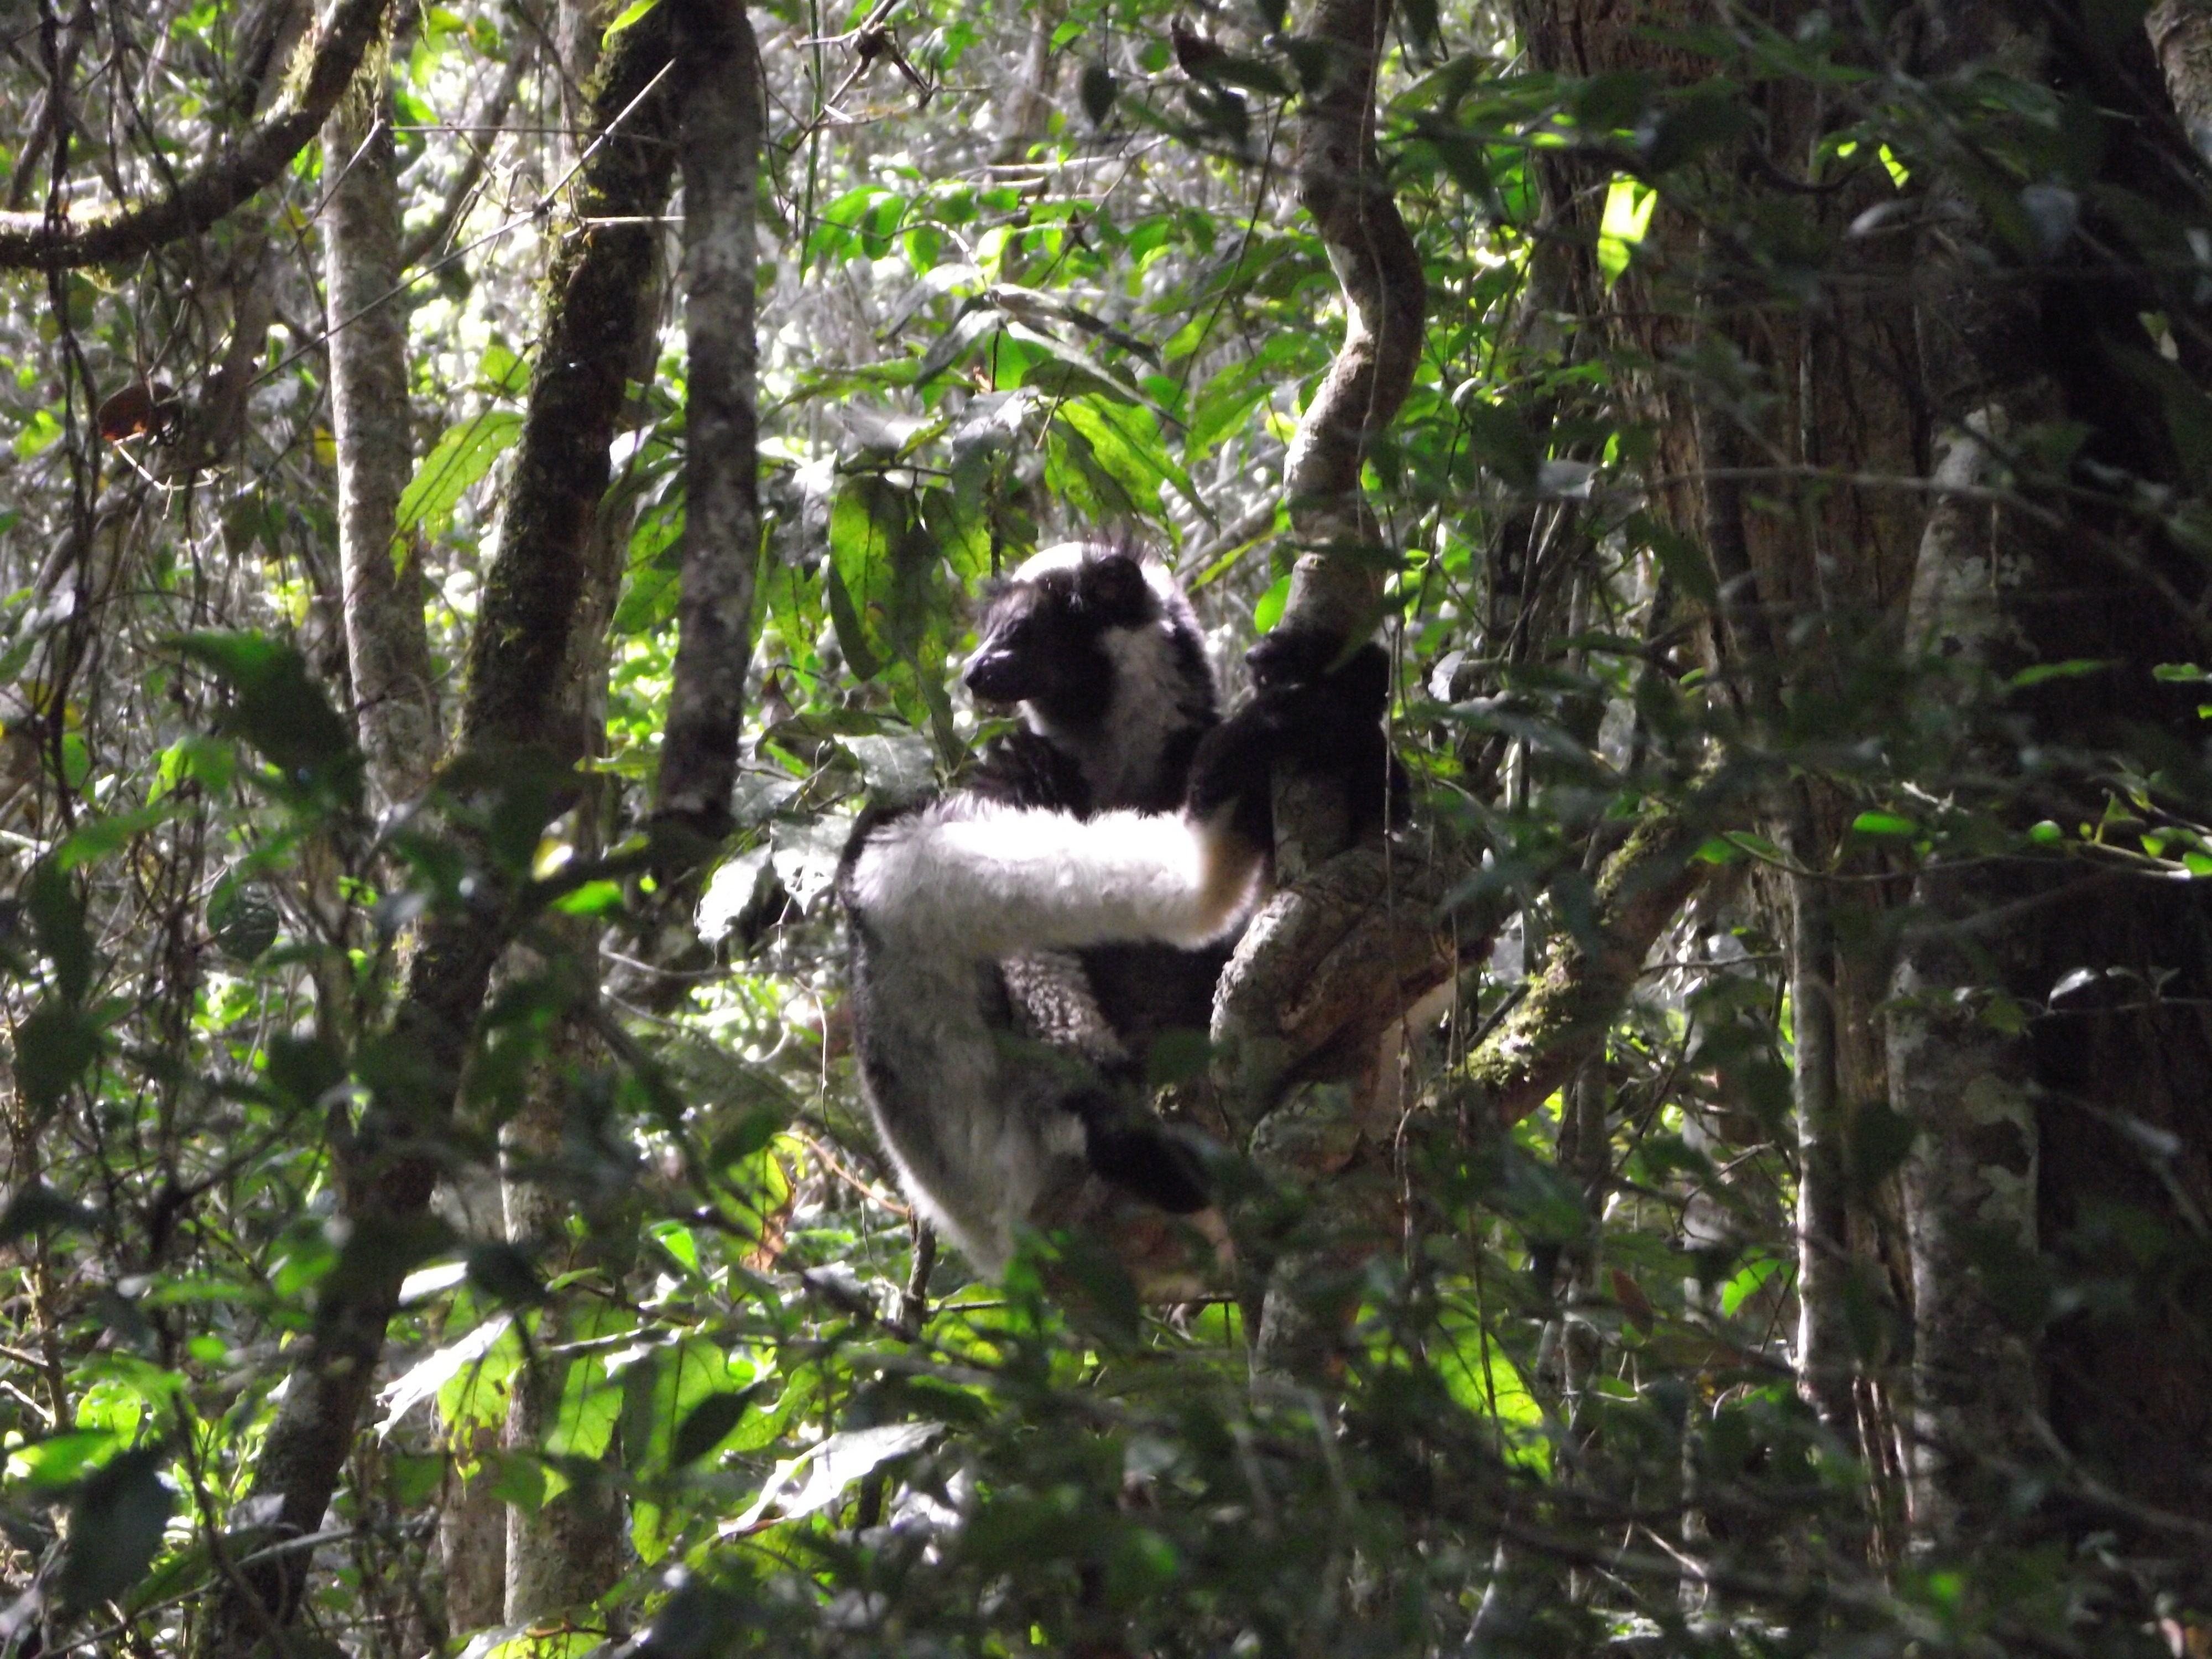
\includegraphics[width=5cm]{articles/Une-boucle-du-cote-vert/DSCF0386.JPG}
\smallbreak

On continu la promenade dans le parc, et je vois alors le lémure bambou, qui mange devinez quoi.. Je reste un certain temps à l'observer puis à le filmer, bien marrant ce petit lémure !

\smallbreak\smallbreak
\hspace*{-0.65cm}
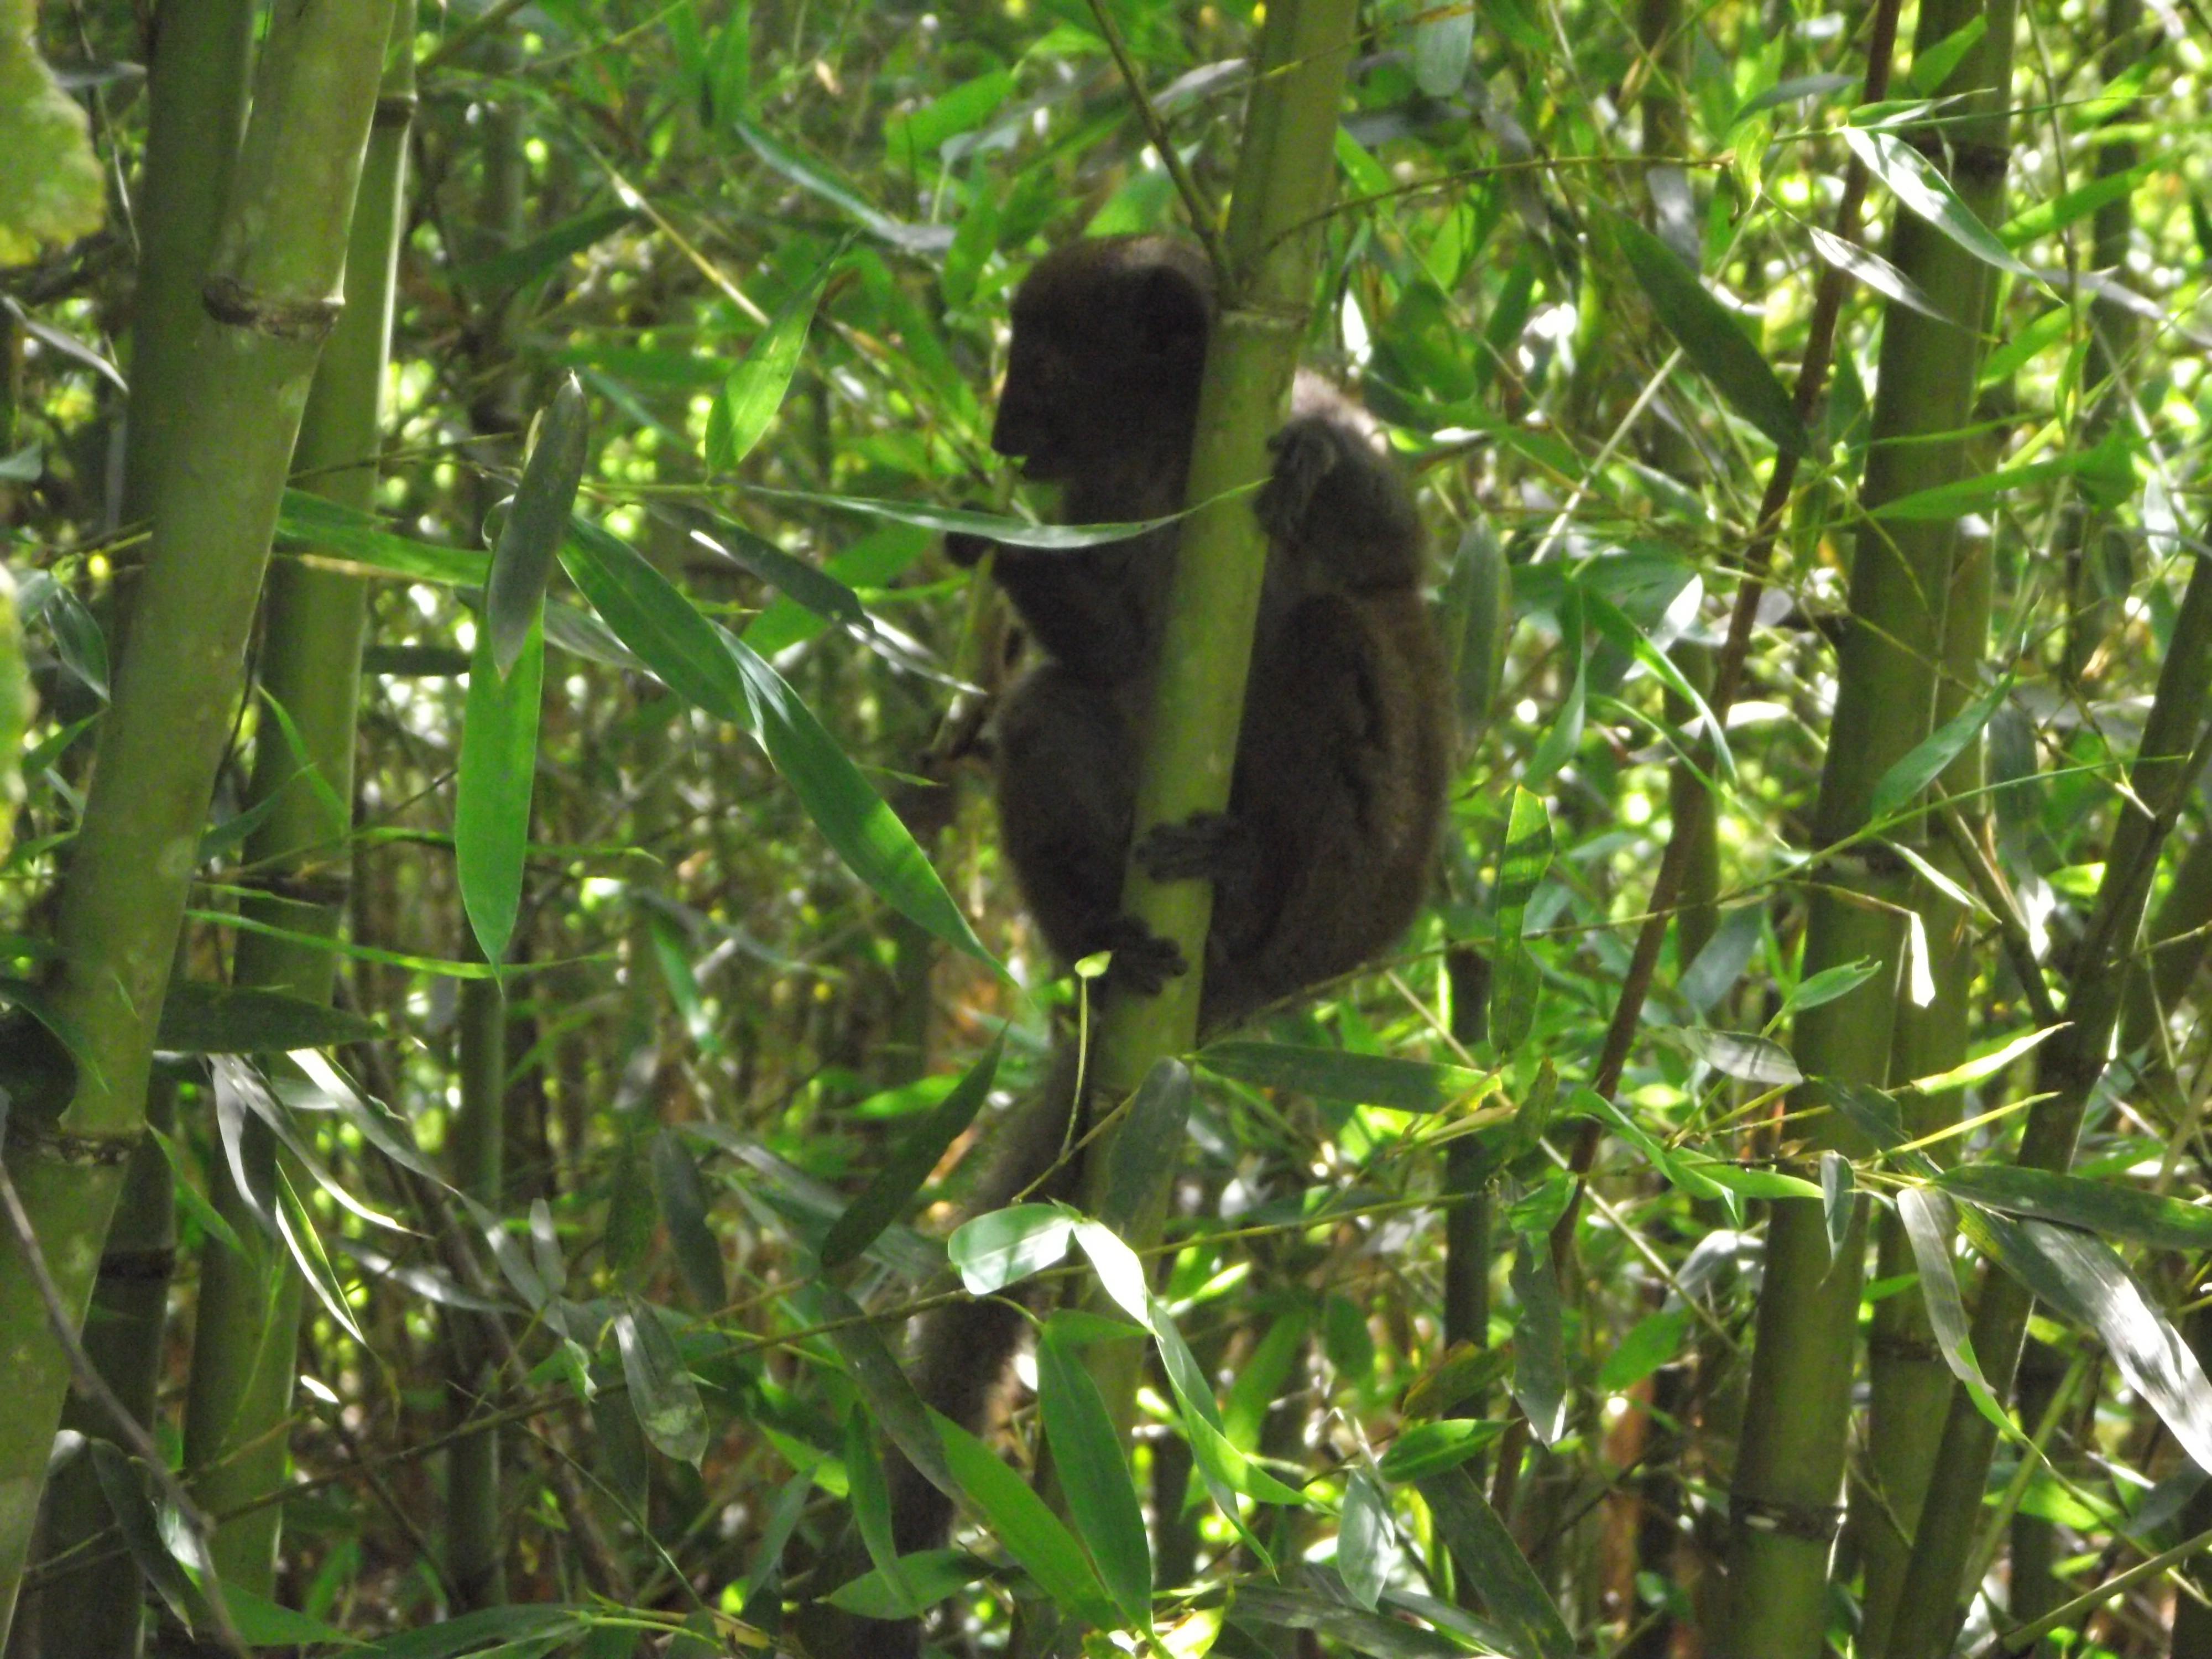
\includegraphics[width=5cm]{articles/Une-boucle-du-cote-vert/DSCF0395.JPG}
\smallbreak

Une fois finie la visite du parc me voici de retour à Tana le soir, puis direction le nord à partir du lendemain. La première escale sera Maevatanana.. oh et puis non il semble qu'il n'y ai pas beaucoup d'activité, vamos a Mahajunga direct, c'est parti pour 13h de taxi brousse pour arriver dans cette ville au bord de mer.

Je me ballade le lendemain, mais la ville semble déserte, en fait on est dimanche et le dimanche à Madagascar certains endroits ont l'allure de ville fantôme. Voici quelques pousse-pousses devant les boutres des pêcheurs, sur le port.

\smallbreak\smallbreak
\hspace*{-0.65cm}
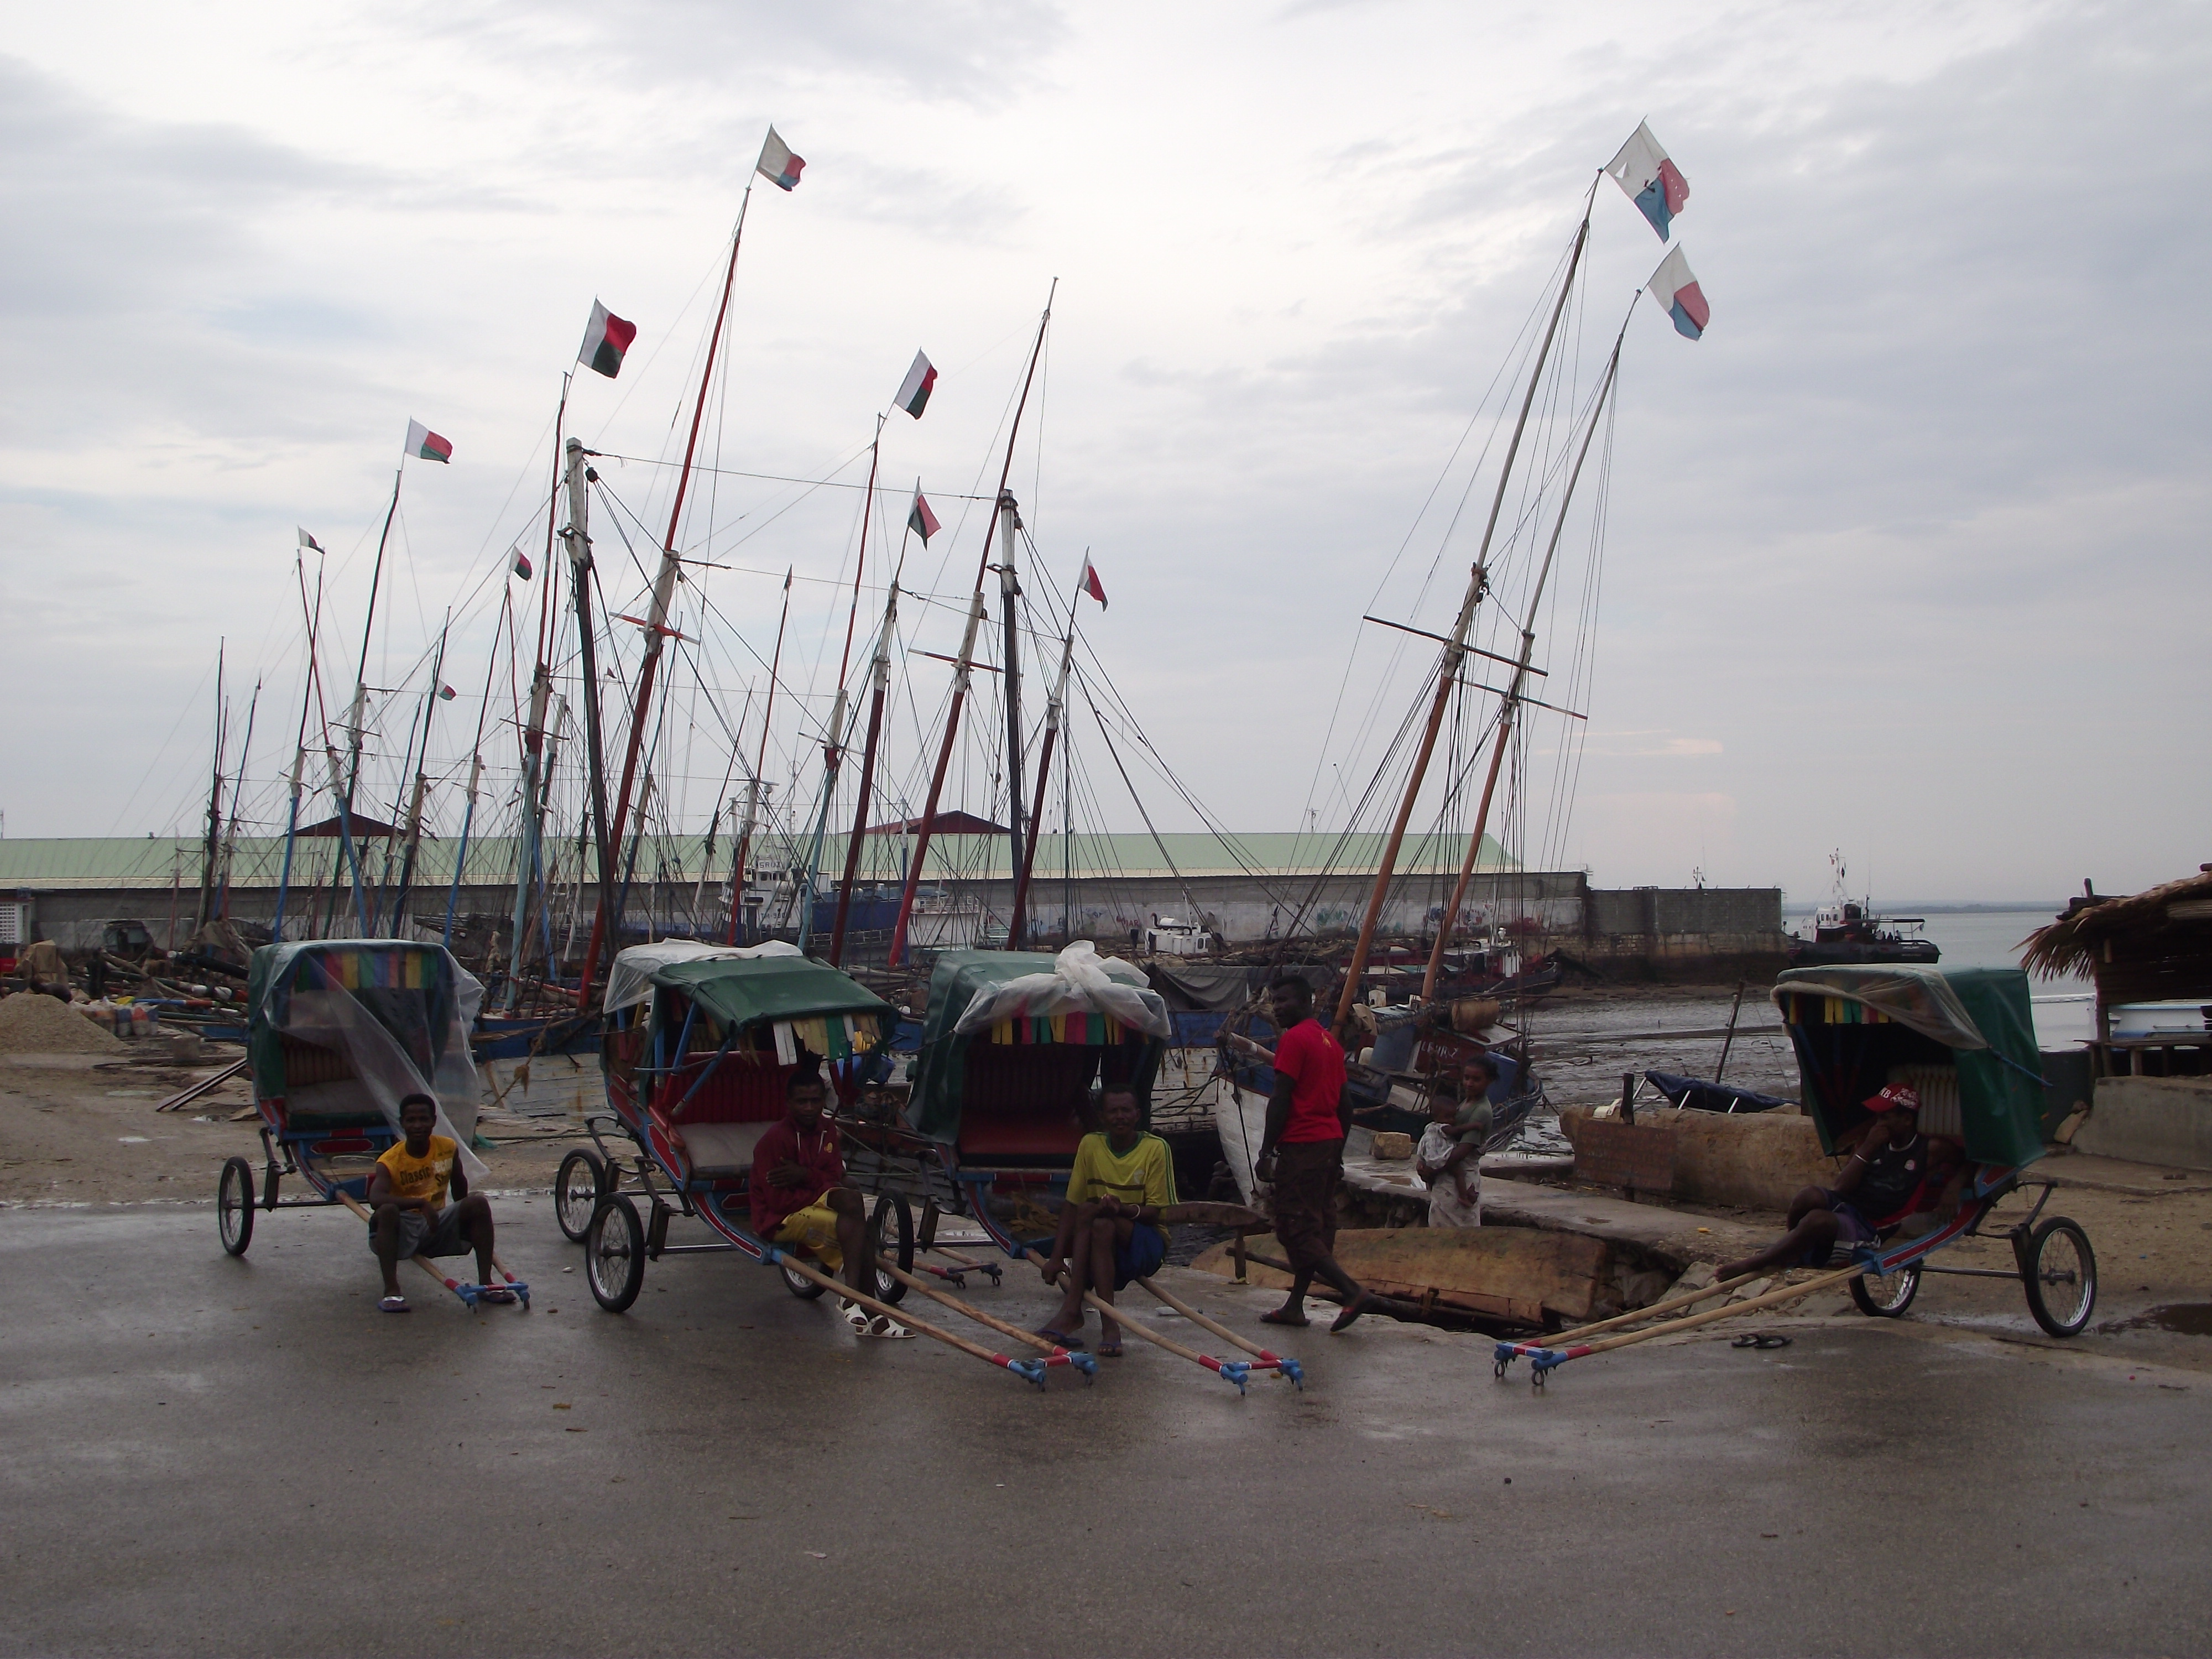
\includegraphics[width=5cm]{articles/Une-boucle-du-cote-vert/DSCF0403.JPG}
\smallbreak

Puis un peu plus loin sur la jetée je vois une pirogue qui rentre.

\smallbreak\smallbreak
\hspace*{-0.65cm}
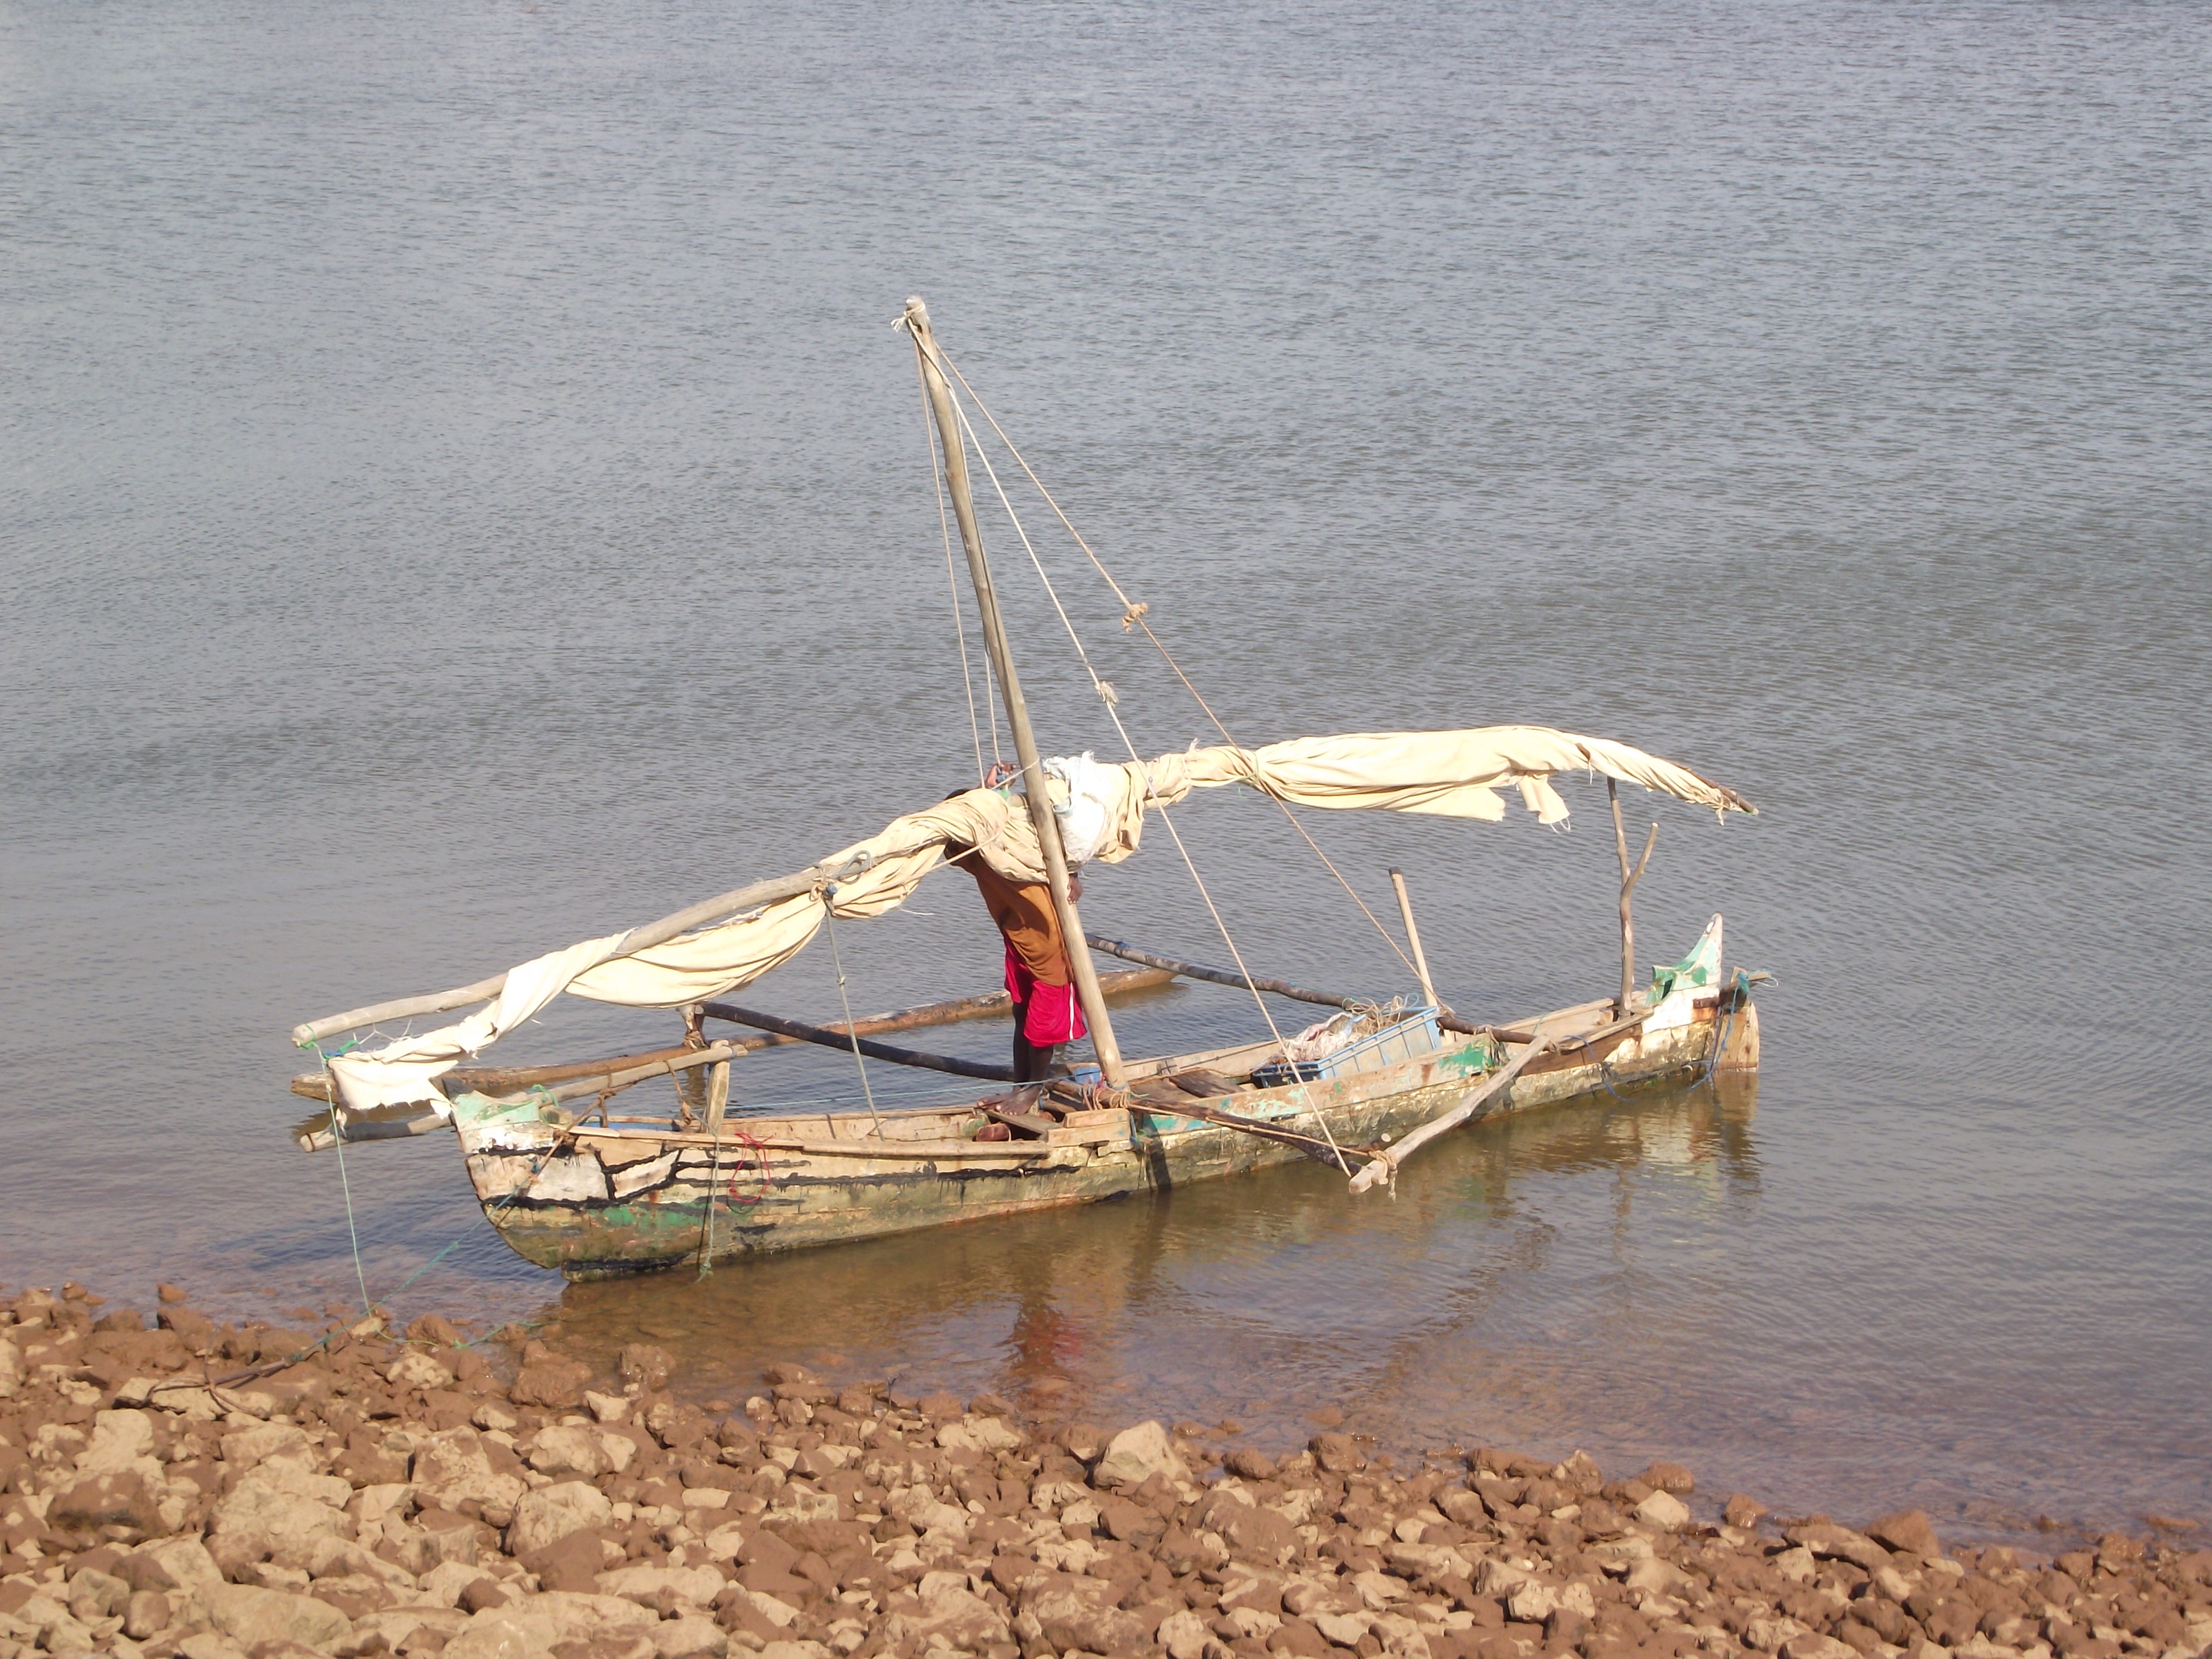
\includegraphics[width=5cm]{articles/Une-boucle-du-cote-vert/DSCF0398.JPG}
\smallbreak

OK, sympa cette ville mais je n'ai pas envie d'y rester plus que ça. J'appelle alors Anthony, un français de l'Ardèche, que j'avais rencontré en début de voyage à Antsirabe, on s'était convenus de se donner des nouvelles vers la fin de ma boucle car nous serions alors tous les deux dans le nord du pays, l'occasion de voyager quelques jours ensembles. Et la, le hasard en voyage n'existe pas, il est en route pour Mahajunga et arrive dans moins d'une heure, cool rasta, on va pouvoir tracer le chemin ensembles.

Nous partons alors pour Nosy Be, ZE place touristique de Madagascar. Nous y passons deux jours, louons des motos pour faire le tour de l'île qui a certes, quelques belles plages, mais qui a surtout beaucoup trop de vazahas, et pas du meilleur spécimen. Il s'agit là du vieux blanc de 50 ans venu en colon profiter du rhum, des plages, et de certaines autres spécificités locales (certains comprendront). Voici une plage du nord de Nosy Be.

\smallbreak\smallbreak
\hspace*{-0.65cm}
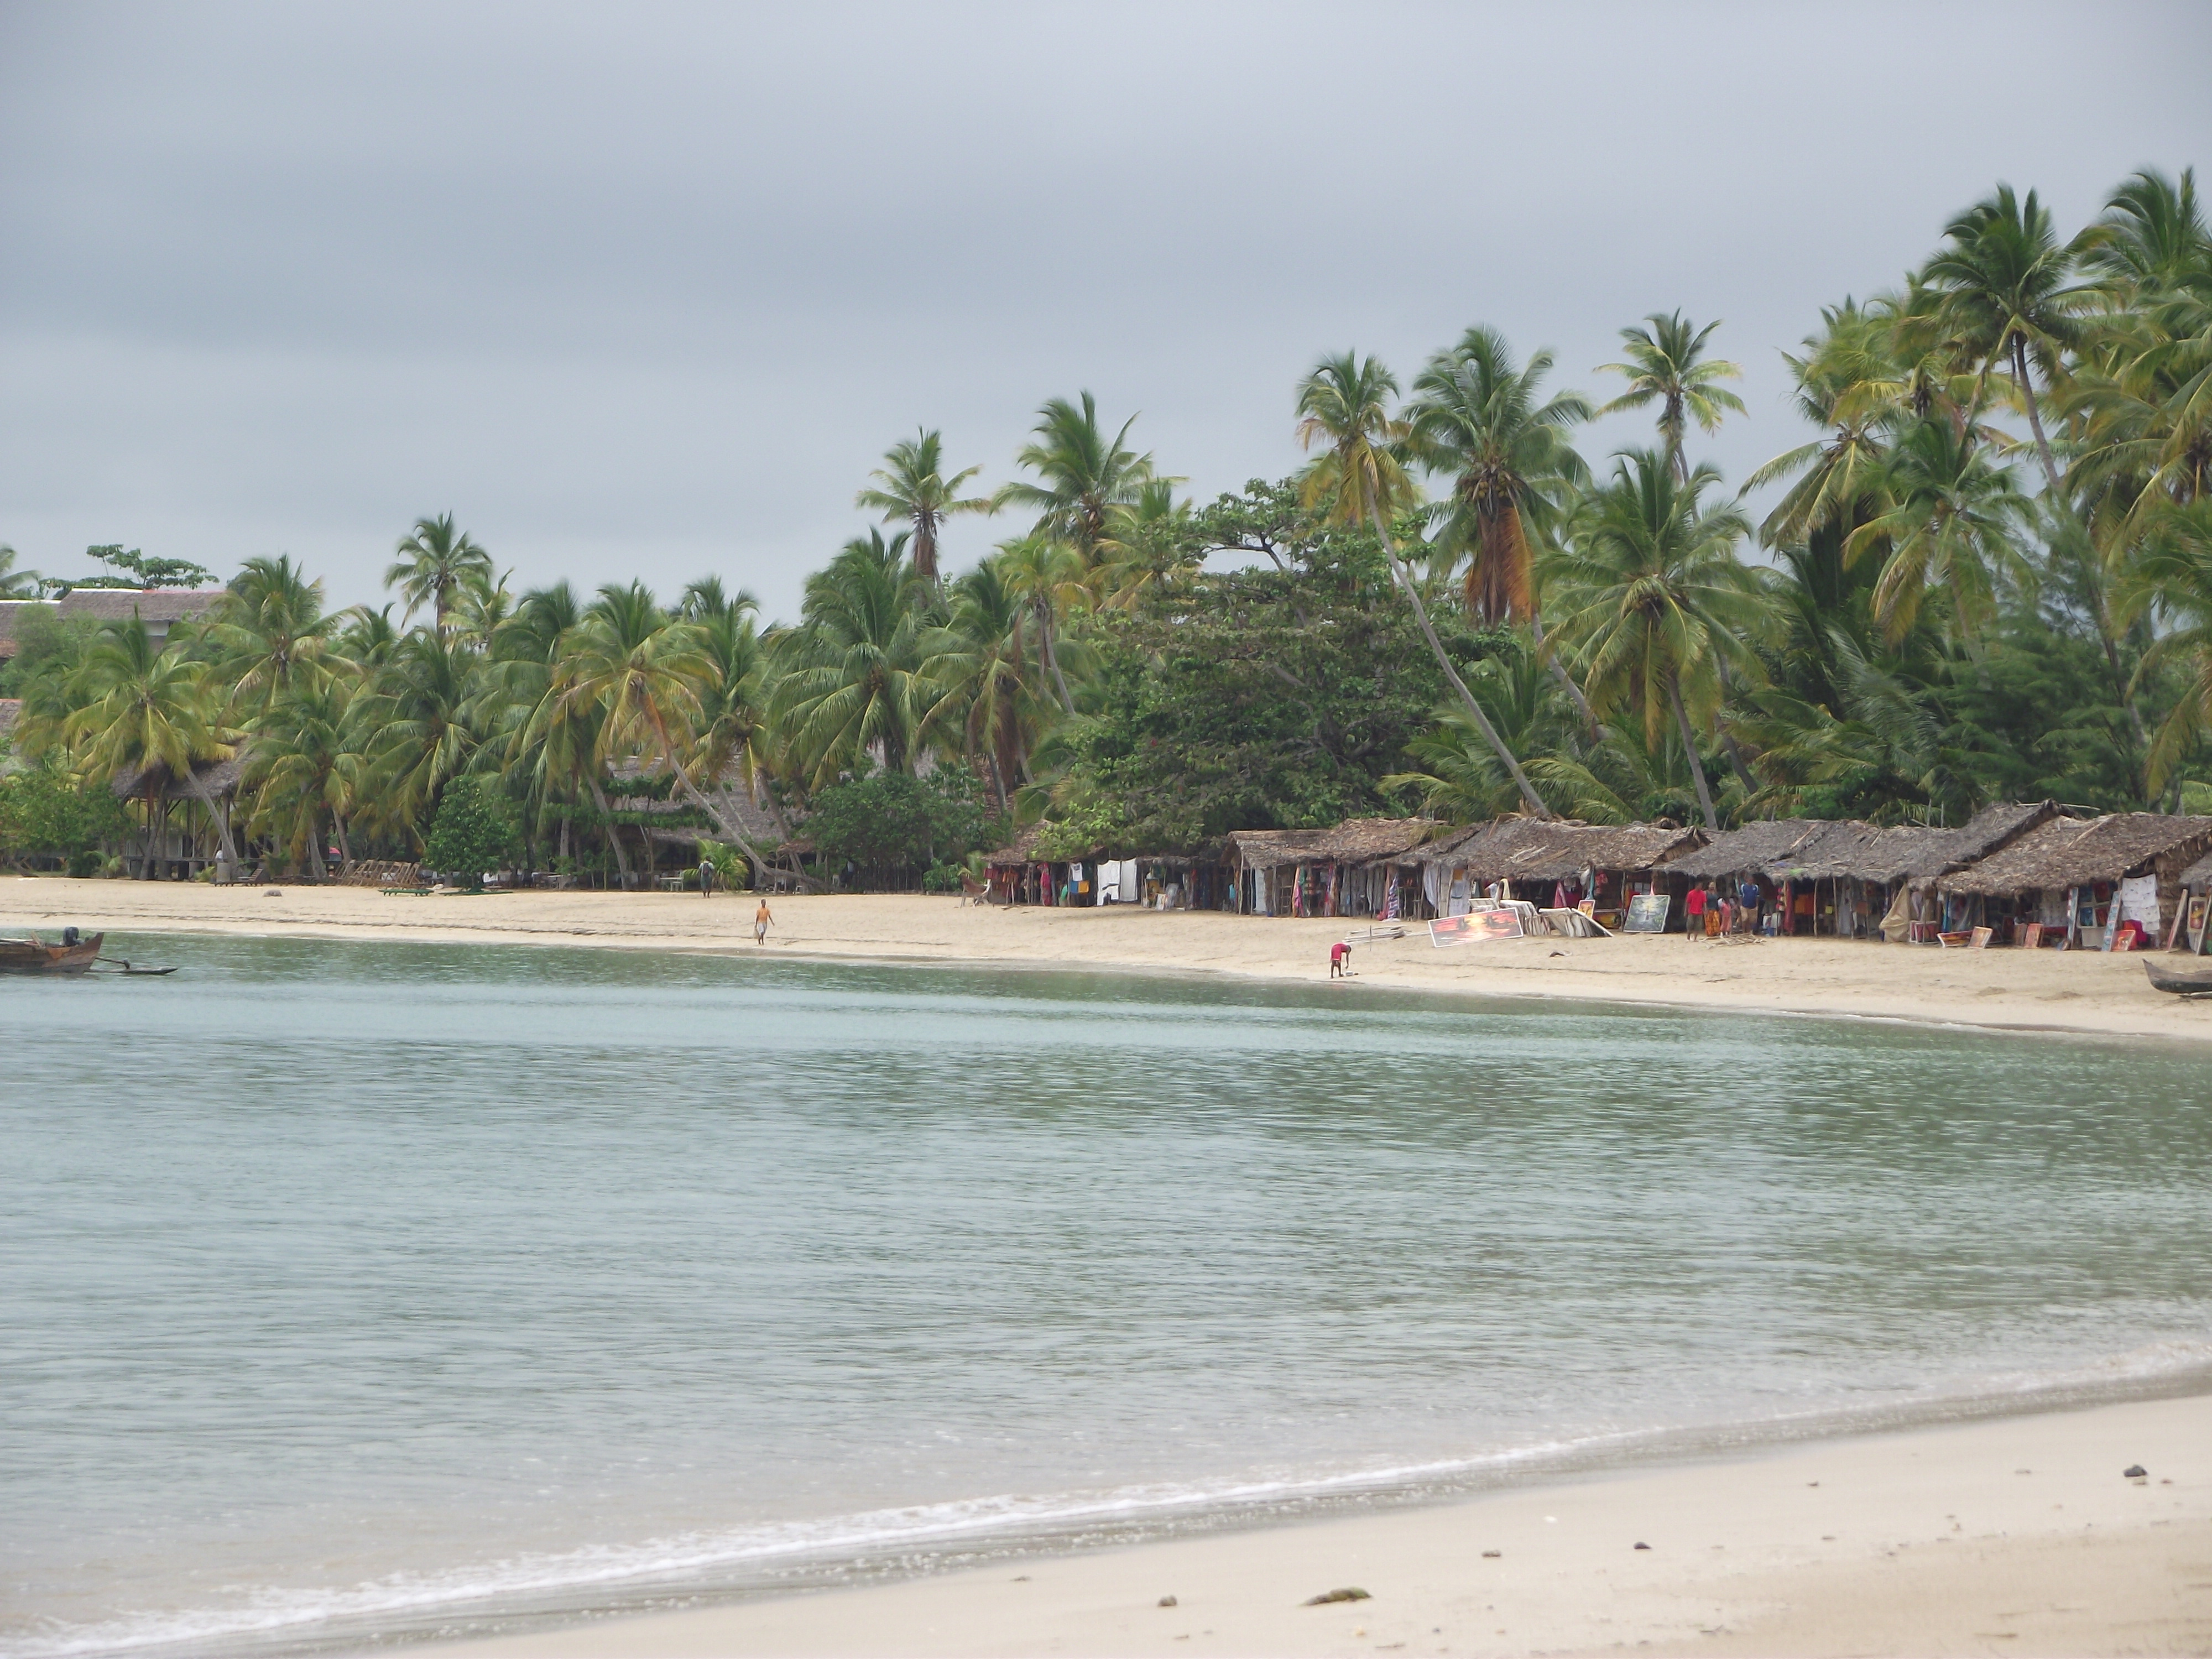
\includegraphics[width=5cm]{articles/Une-boucle-du-cote-vert/DSCF0418.JPG}
\smallbreak

Puis nous mettons le cap vers Nosy Komba, ile toute voisine et beaucoup plus authentique. Voici une pirogue croisée durant la traversée.

\smallbreak\smallbreak
\hspace*{-0.65cm}
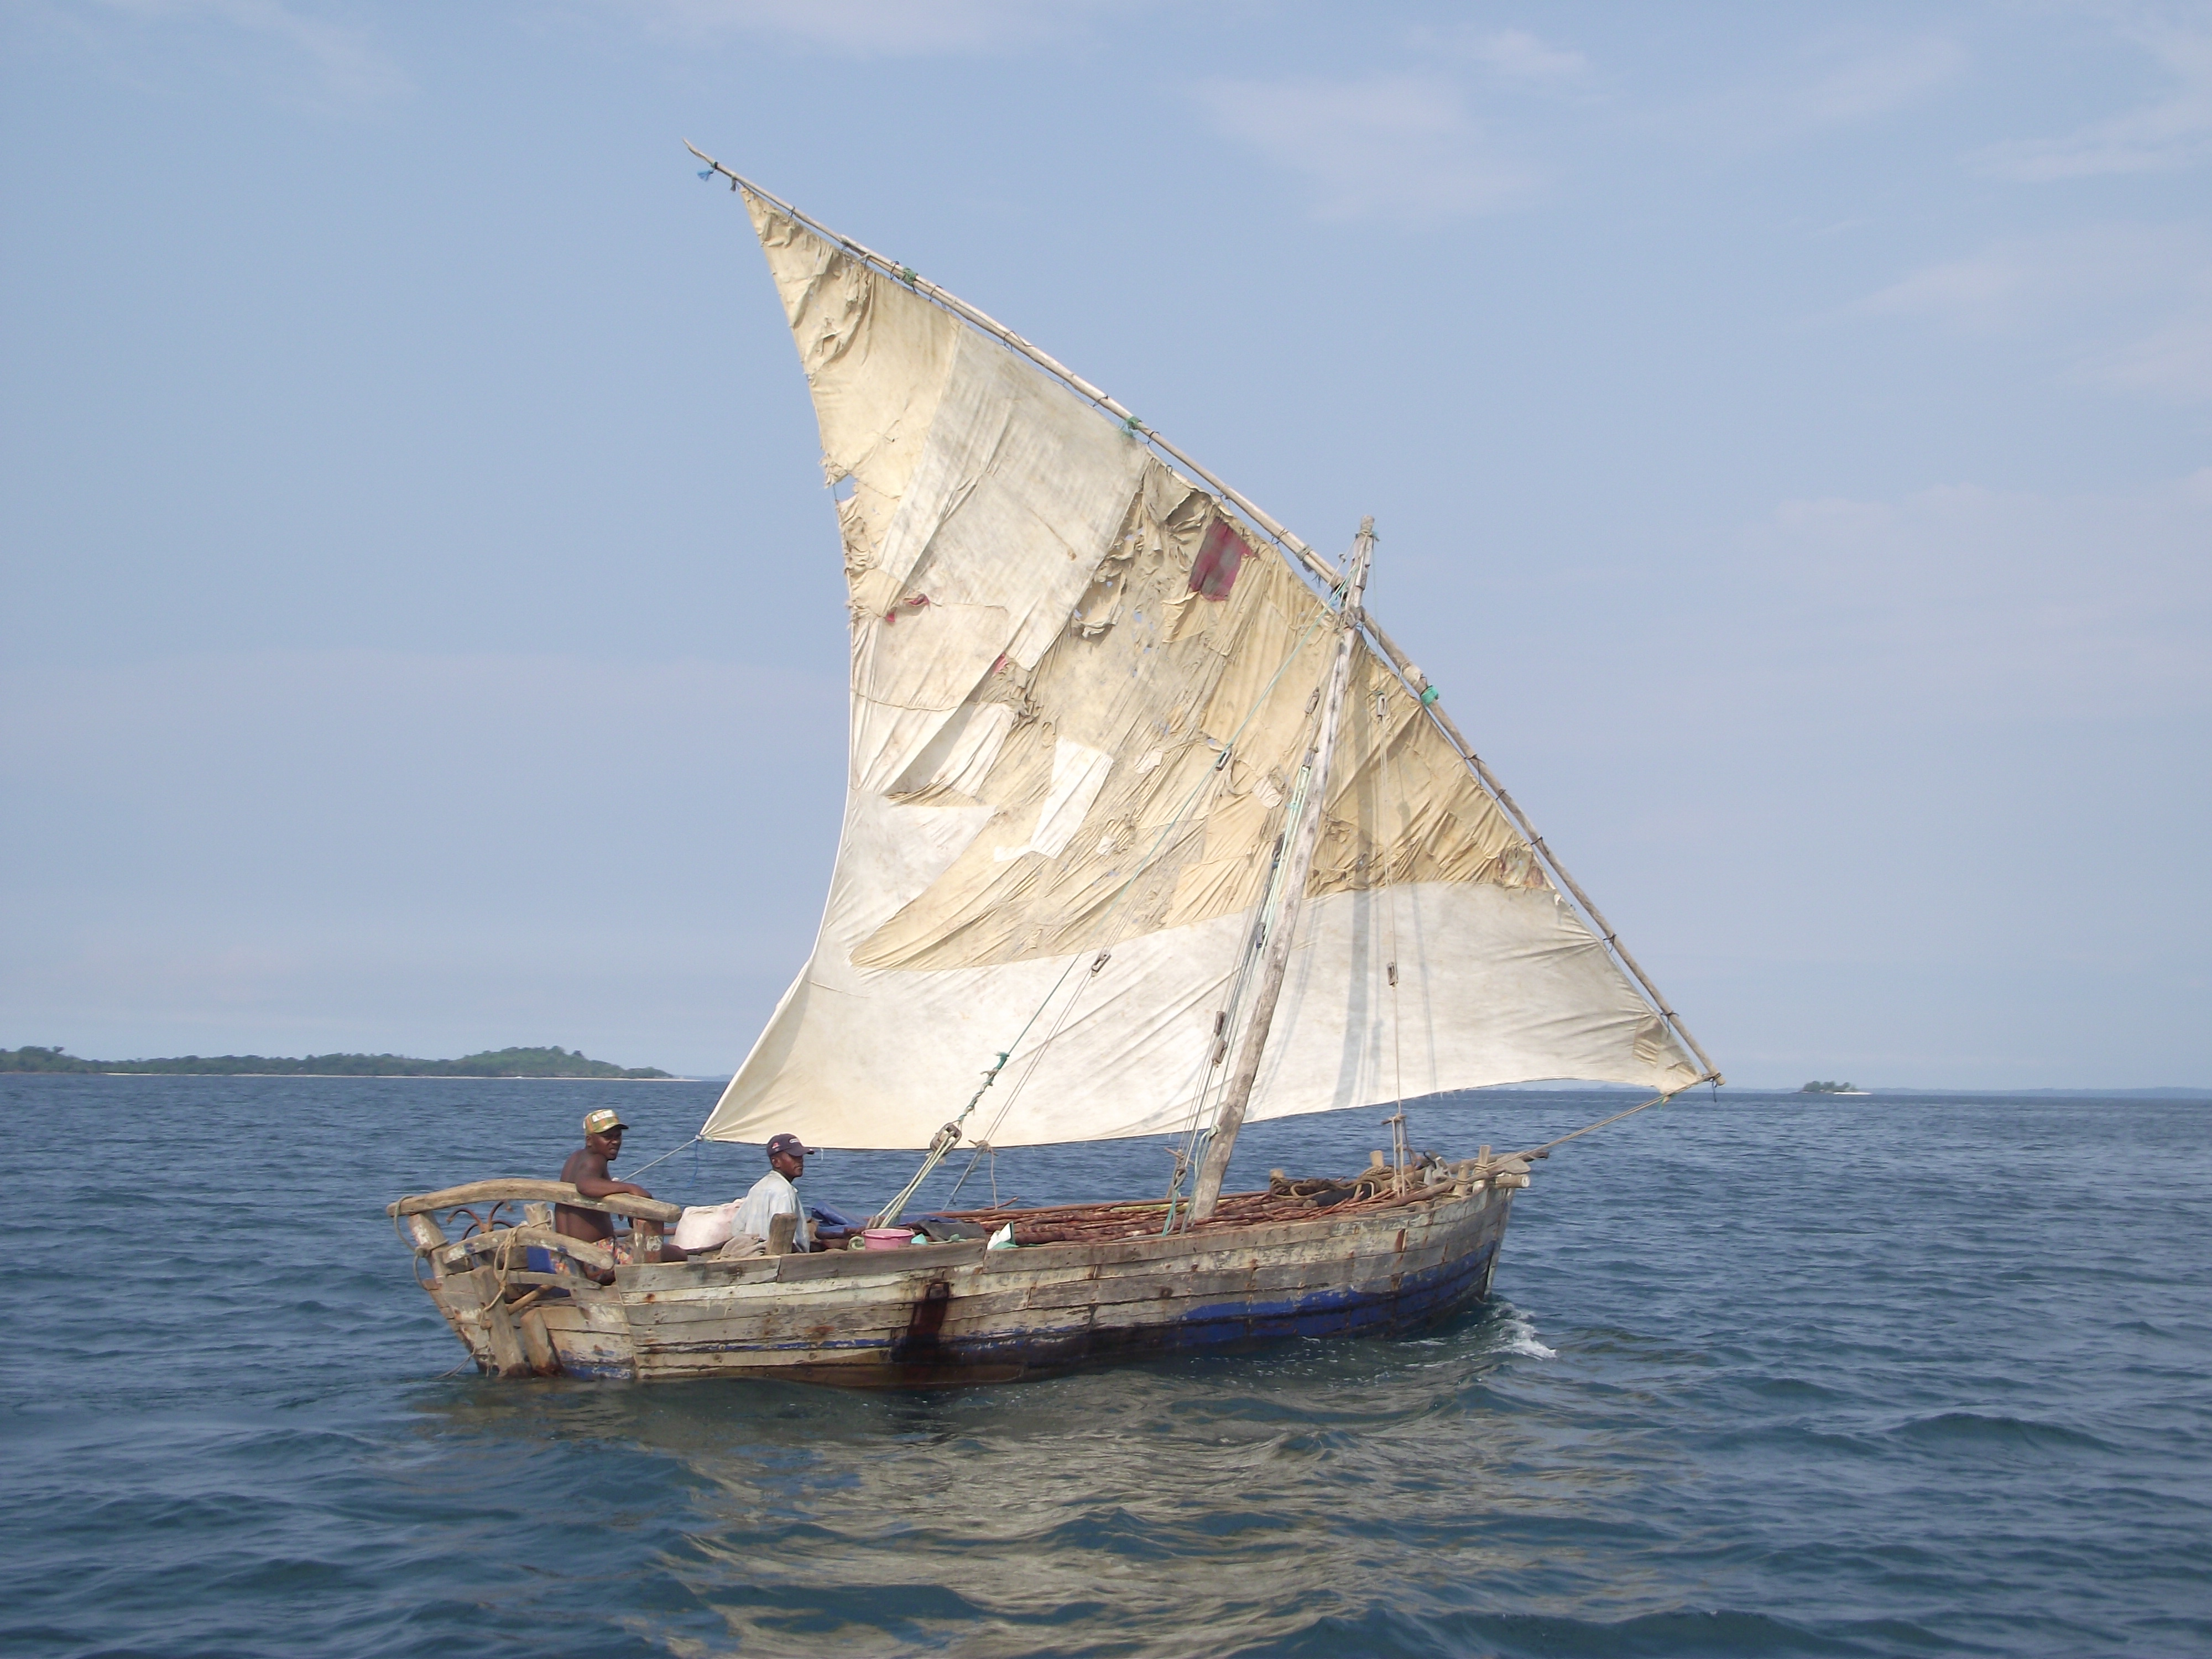
\includegraphics[width=5cm]{articles/Une-boucle-du-cote-vert/DSCF0433.JPG}
\smallbreak

L'occasion de vous montrer un phénomène à Madagascar : dans tout le pays, certaines femmes se mettent une poudre sur le visage pour se protéger du soleil. L'effet est alors certaines fois étonnant pour l'observateur. Dans le nord du pays, et notamment à Nosy Komba, nous avons rencontré des femmes qui font de ce masque un élément de beauté, l'effet est alors magnifique, j'adore vraiment les deux photos qui suivent..

\smallbreak\smallbreak
\hspace*{-0.65cm}
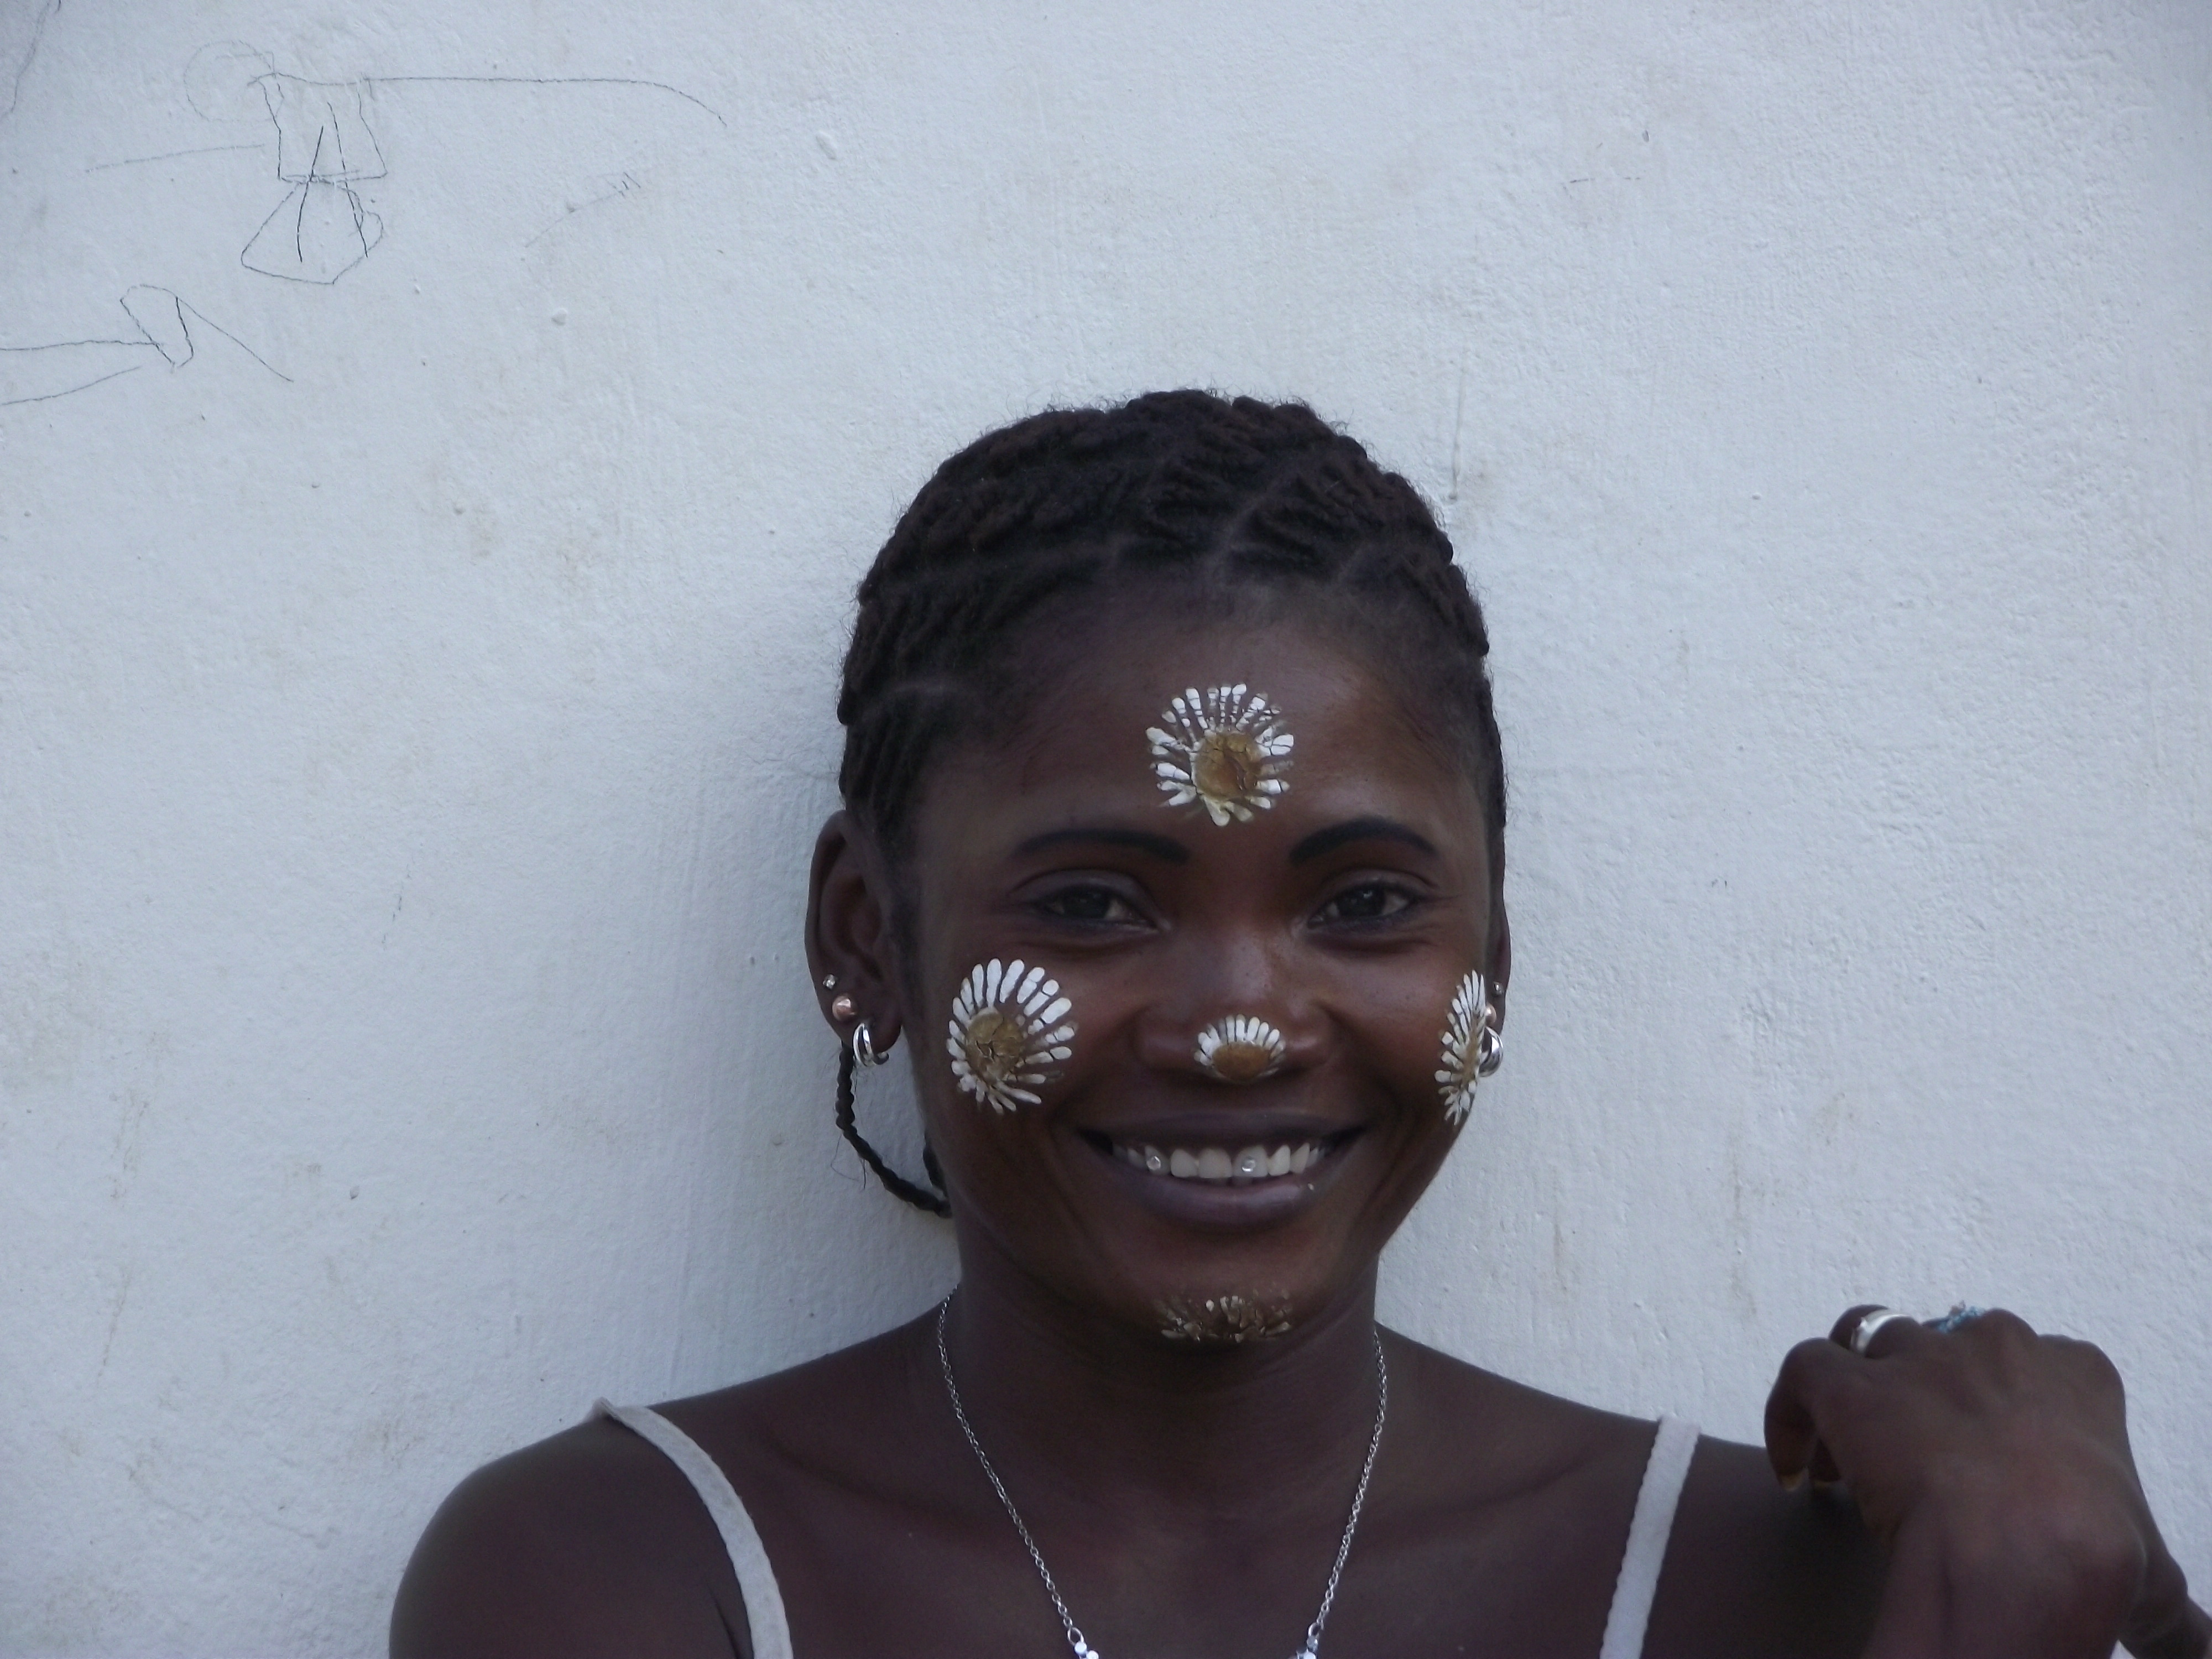
\includegraphics[width=5cm]{articles/Une-boucle-du-cote-vert/DSCF0441.JPG}
\smallbreak

\smallbreak\smallbreak
\hspace*{-0.65cm}
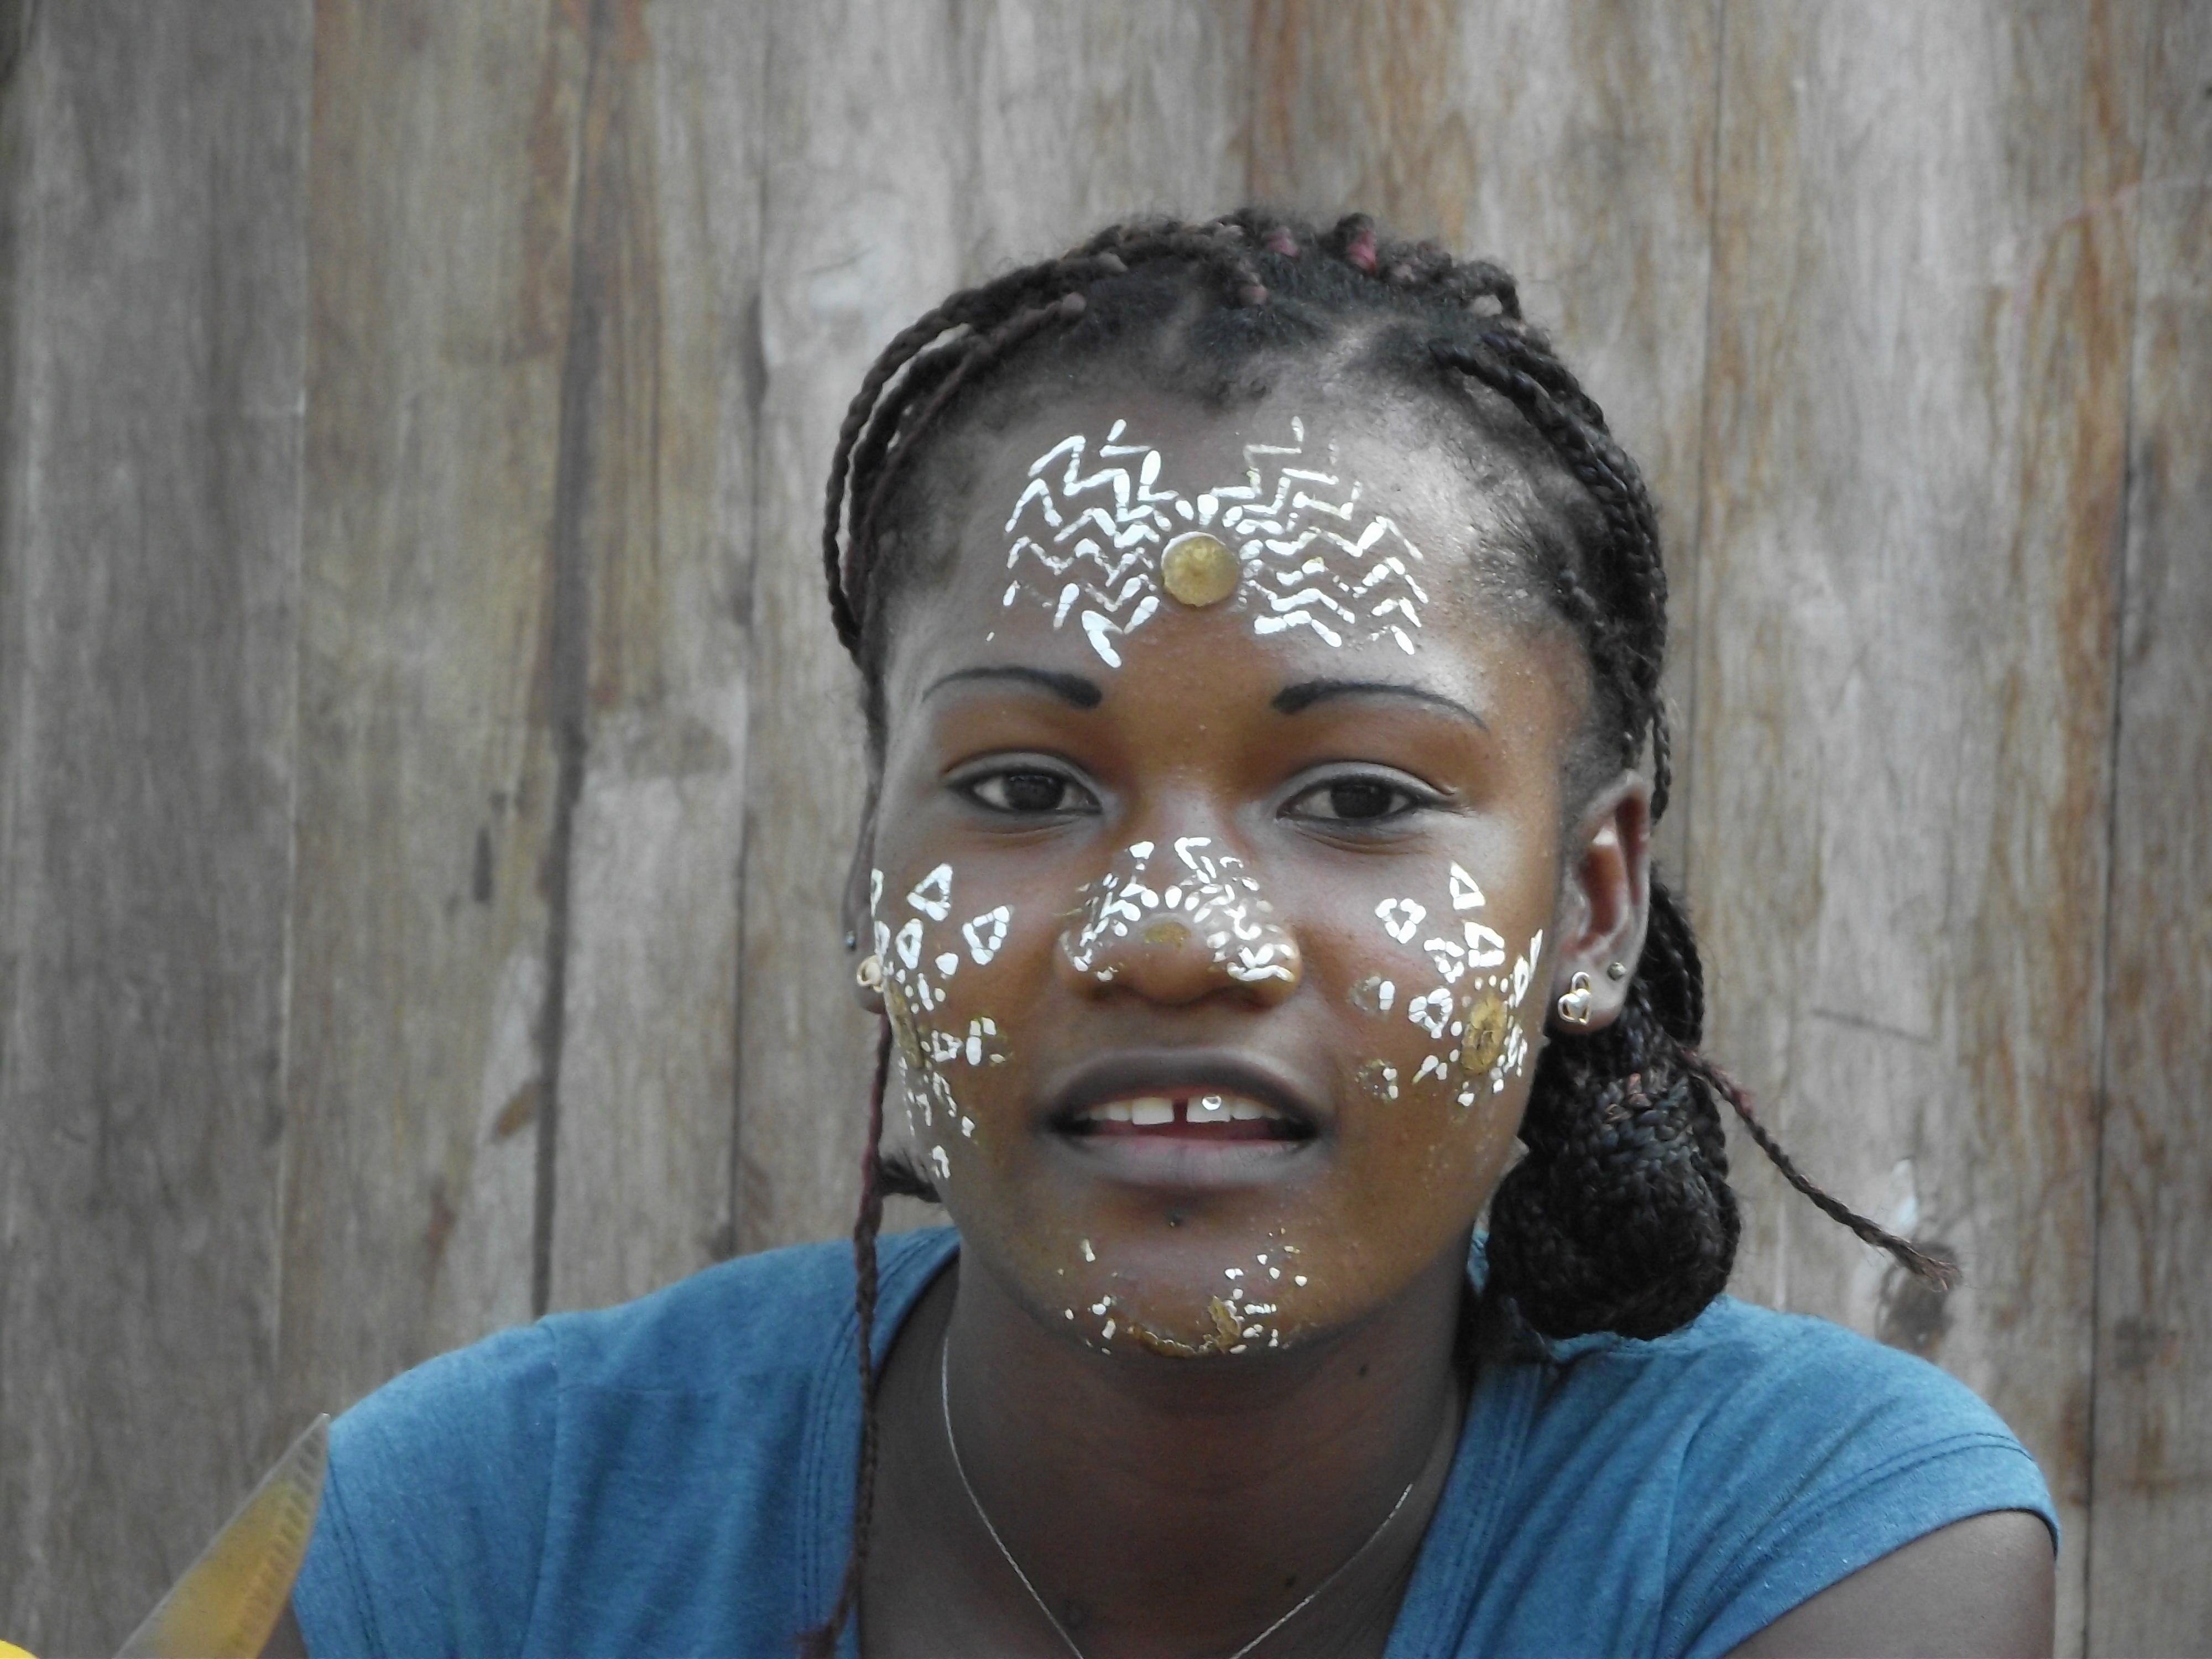
\includegraphics[width=5cm]{articles/Une-boucle-du-cote-vert/DSCF0442.JPG}
\smallbreak

Nosy Komba est aussi l'occasion d'aller faire de la plongée sous marine, histoire d'aller voir ce qui se passe la dessous. Je n'ai pas de photos pour vous le montrer mais la vie sous marine ici est très active, les coraux sont magnifiques, de toutes les couleurs et les poissons tropicaux très variés, j'ai fais deux plongées de 50 minutes chacune, de toute beauté.

Nous quittons alors les îles pour aller à la pointe Nord de Mada, à Diégo Suarez où se termine mon voyage ces jours-ci. Parmi les beaux paysages à aller voir ici se trouve la mer d'Émeraude dont on m'a tant parlé, Anthony et moi louons alors un scooter pour se rendre à Ramena, point de départ des bateaux qui partent à la journée pour visiter cette baie protégée par une barrière de corail.

L'occasion de vous présenter Anthony, à gauche, ainsi que notre cuistot et notre barreur/pêcheur, deux bonhommes bien marrans qui nous ont préparé devinez quoi.. du poisson grillé pêché 10 minutes plus tôt.. mmmmm !!!

\smallbreak\smallbreak
\hspace*{-0.65cm}
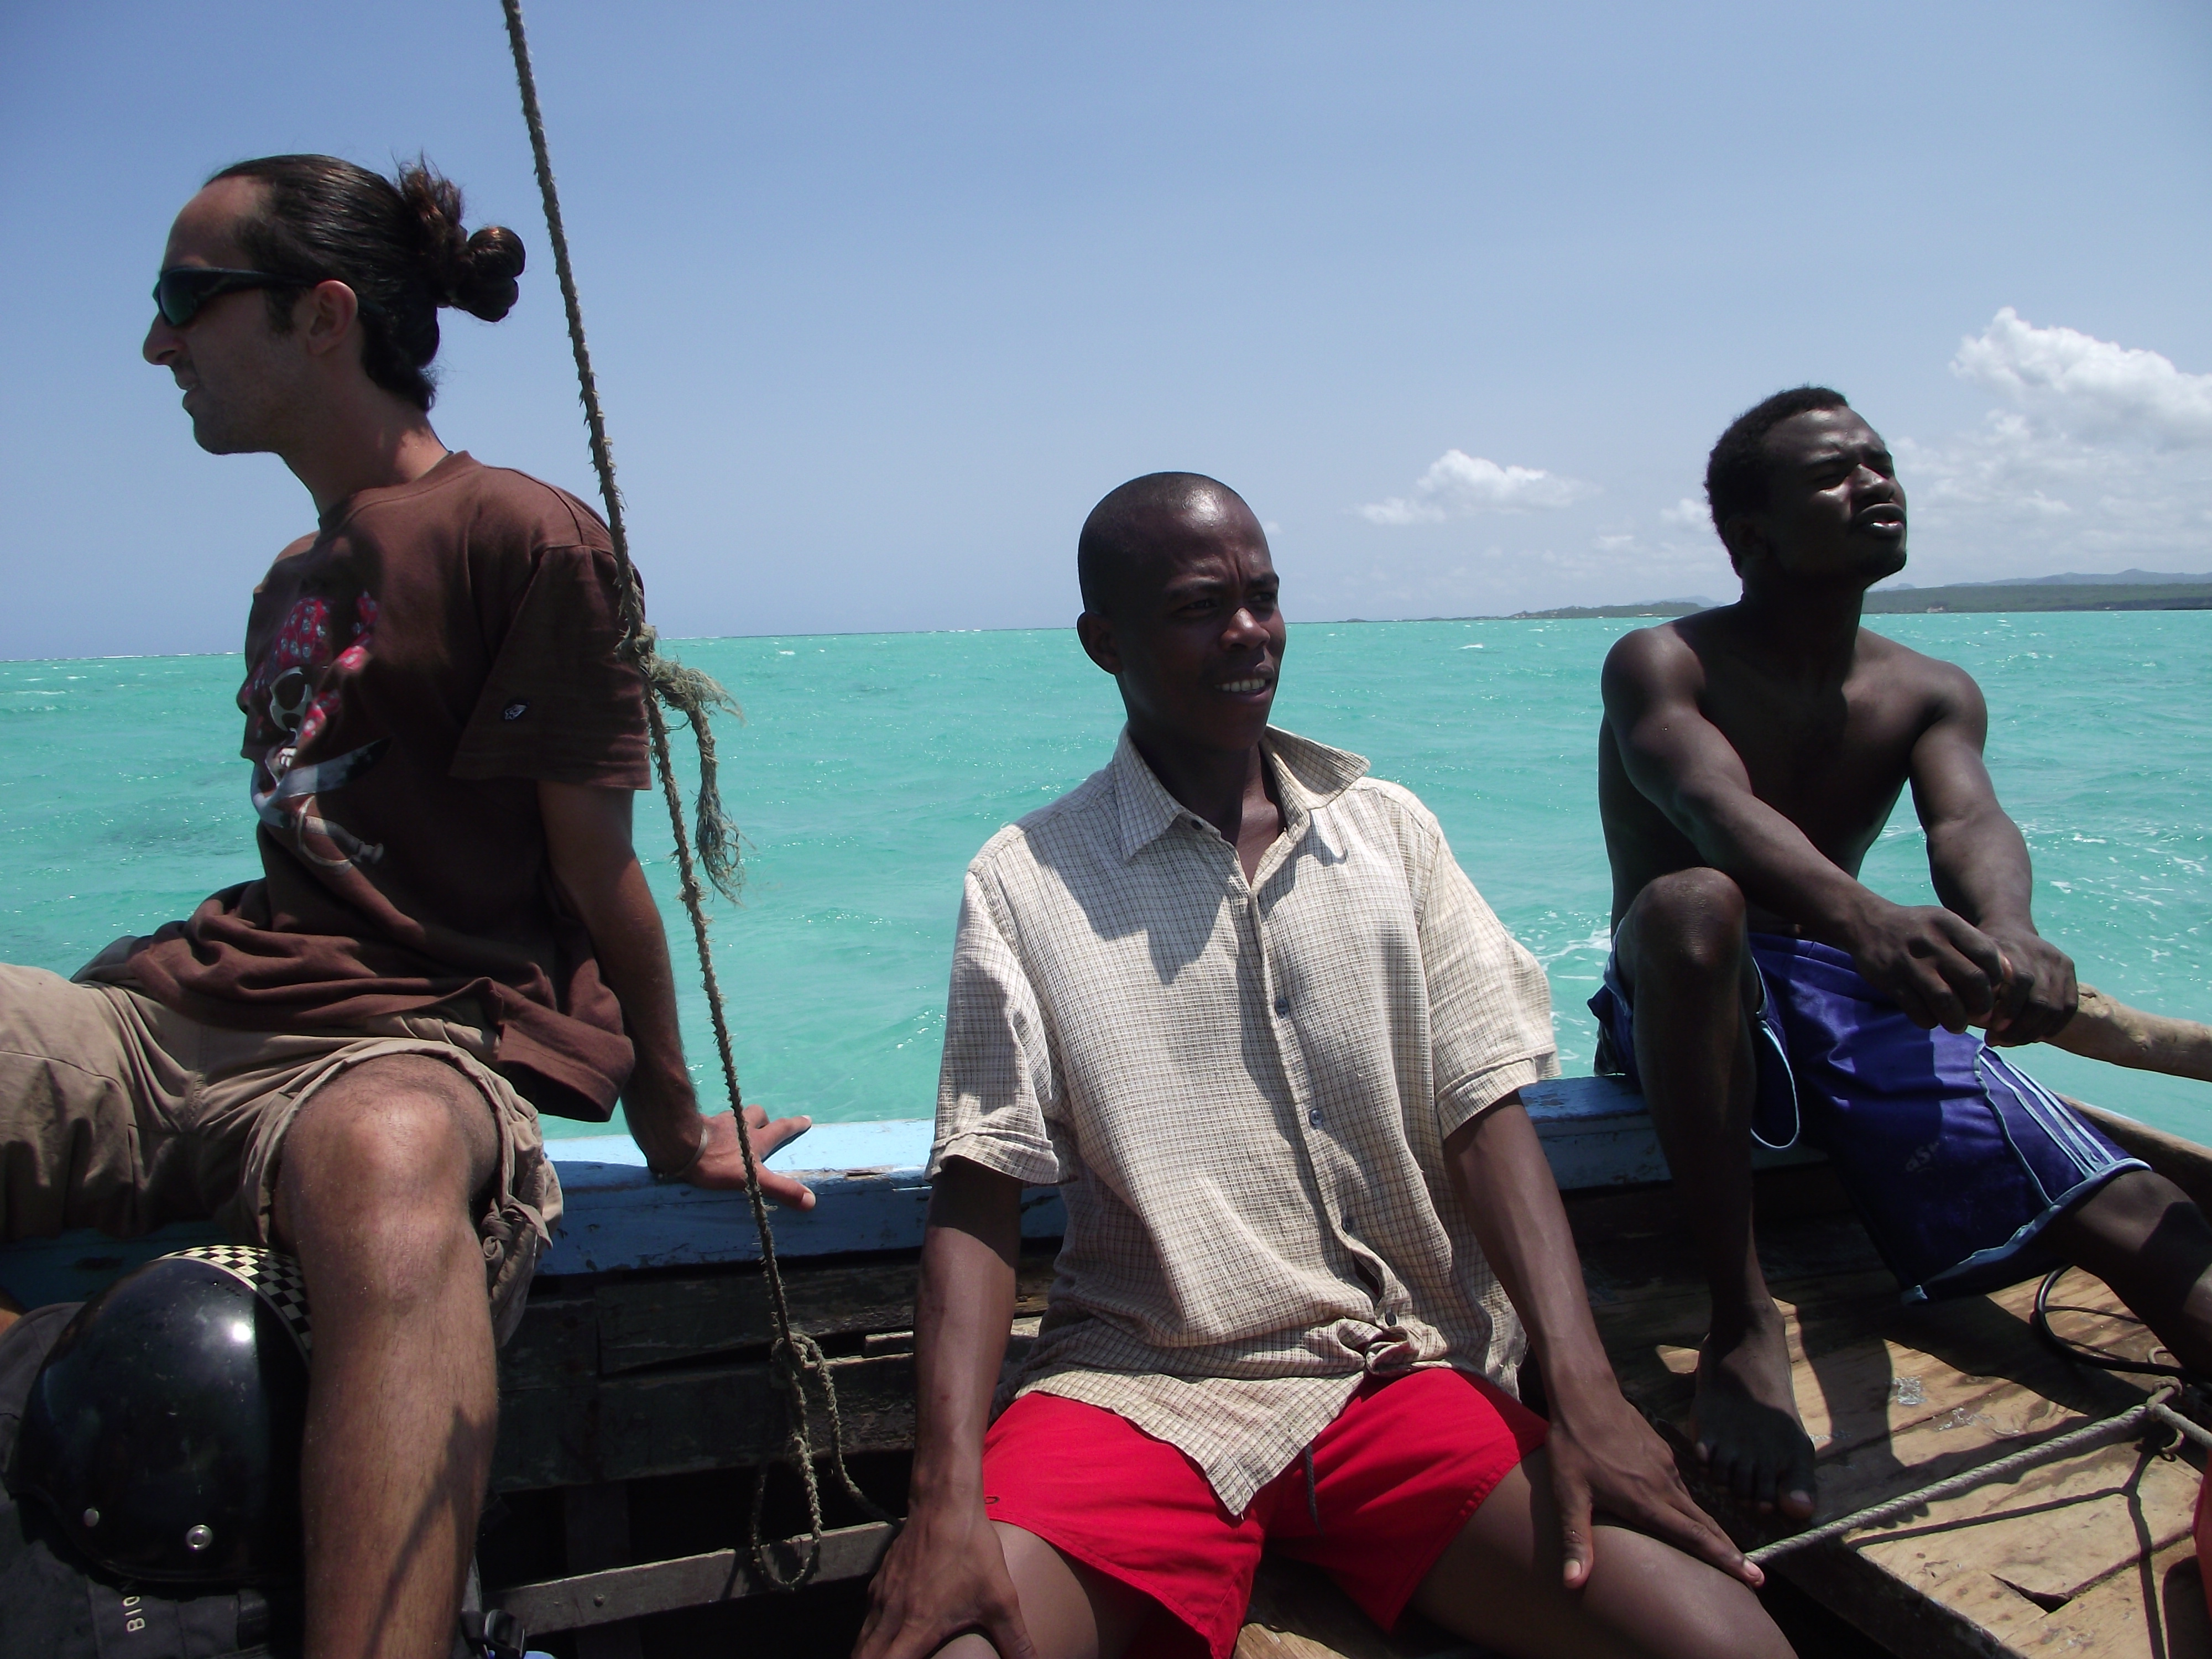
\includegraphics[width=5cm]{articles/Une-boucle-du-cote-vert/DSCF0456.JPG}
\smallbreak

Allez, pour la postérité, "j'y étais !"

\smallbreak\smallbreak
\hspace*{-0.65cm}
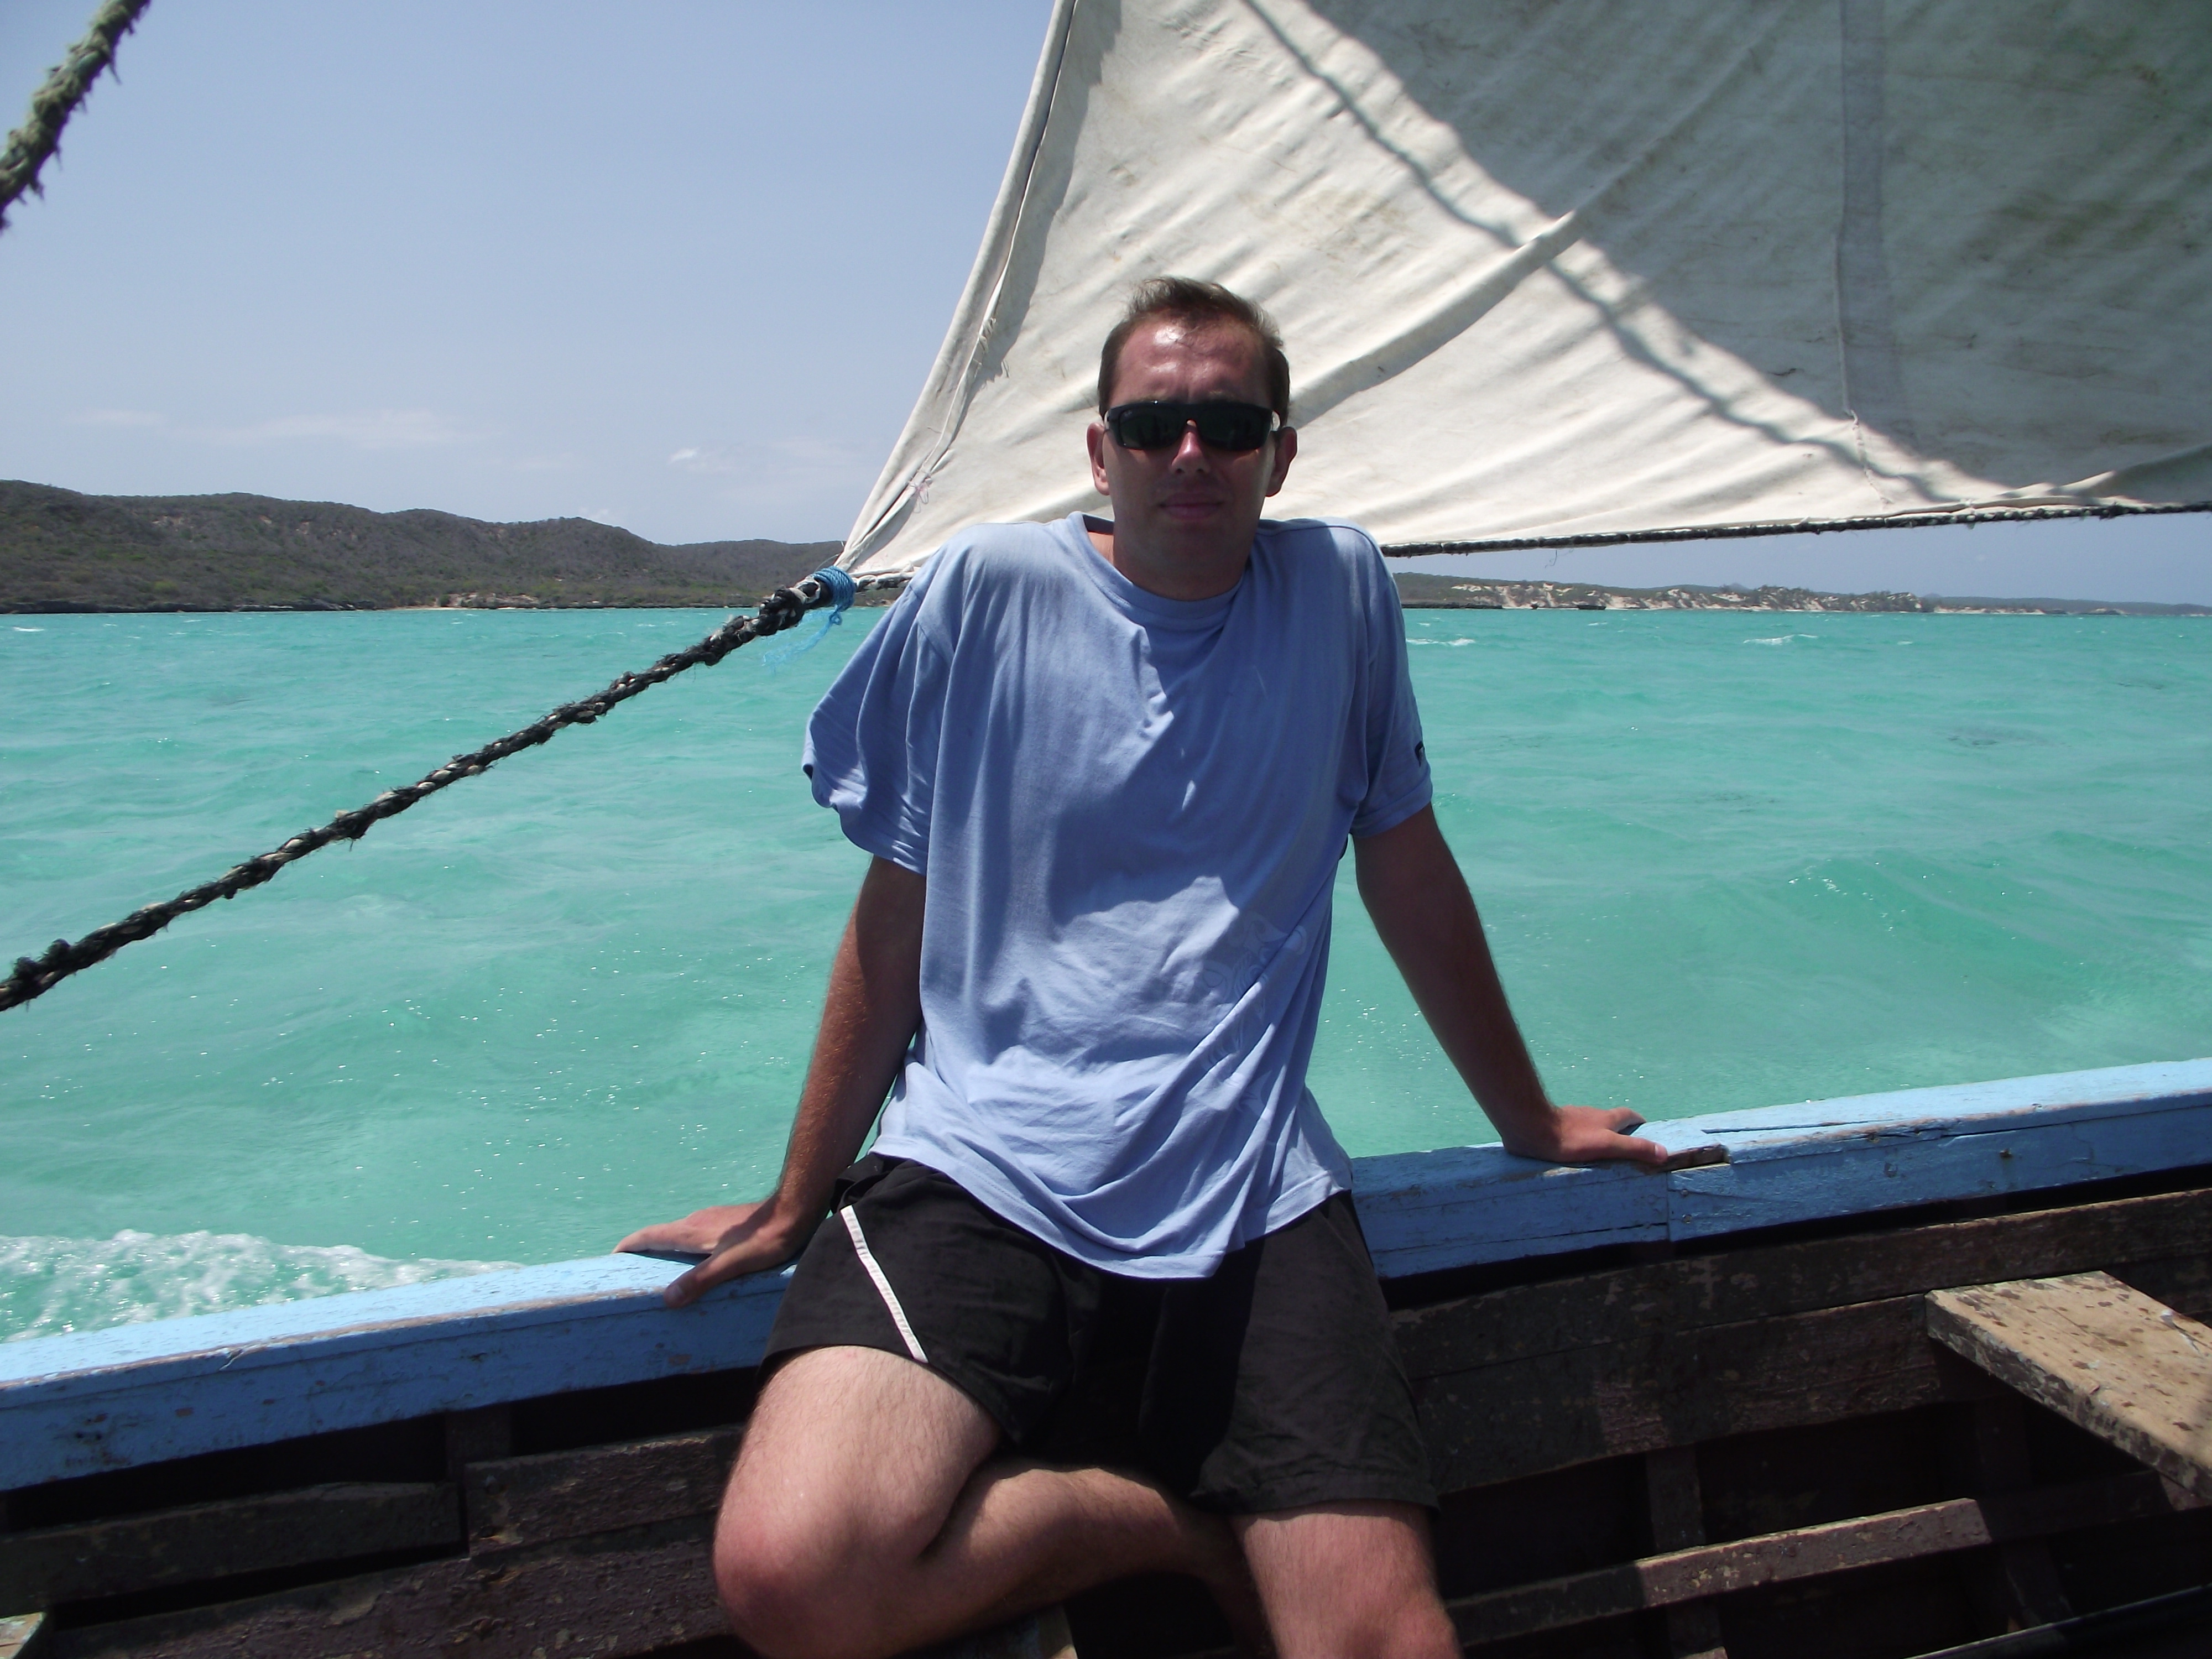
\includegraphics[width=5cm]{articles/Une-boucle-du-cote-vert/DSCF0457.JPG}
\smallbreak

Et on termine ce voyage à Madagsacar par une petite sieste, l'occasion de faire bon usage du cadeau d'au revoir de la conv'tek'team du tonnerre, merci à vous..

\smallbreak\smallbreak
\hspace*{-0.65cm}
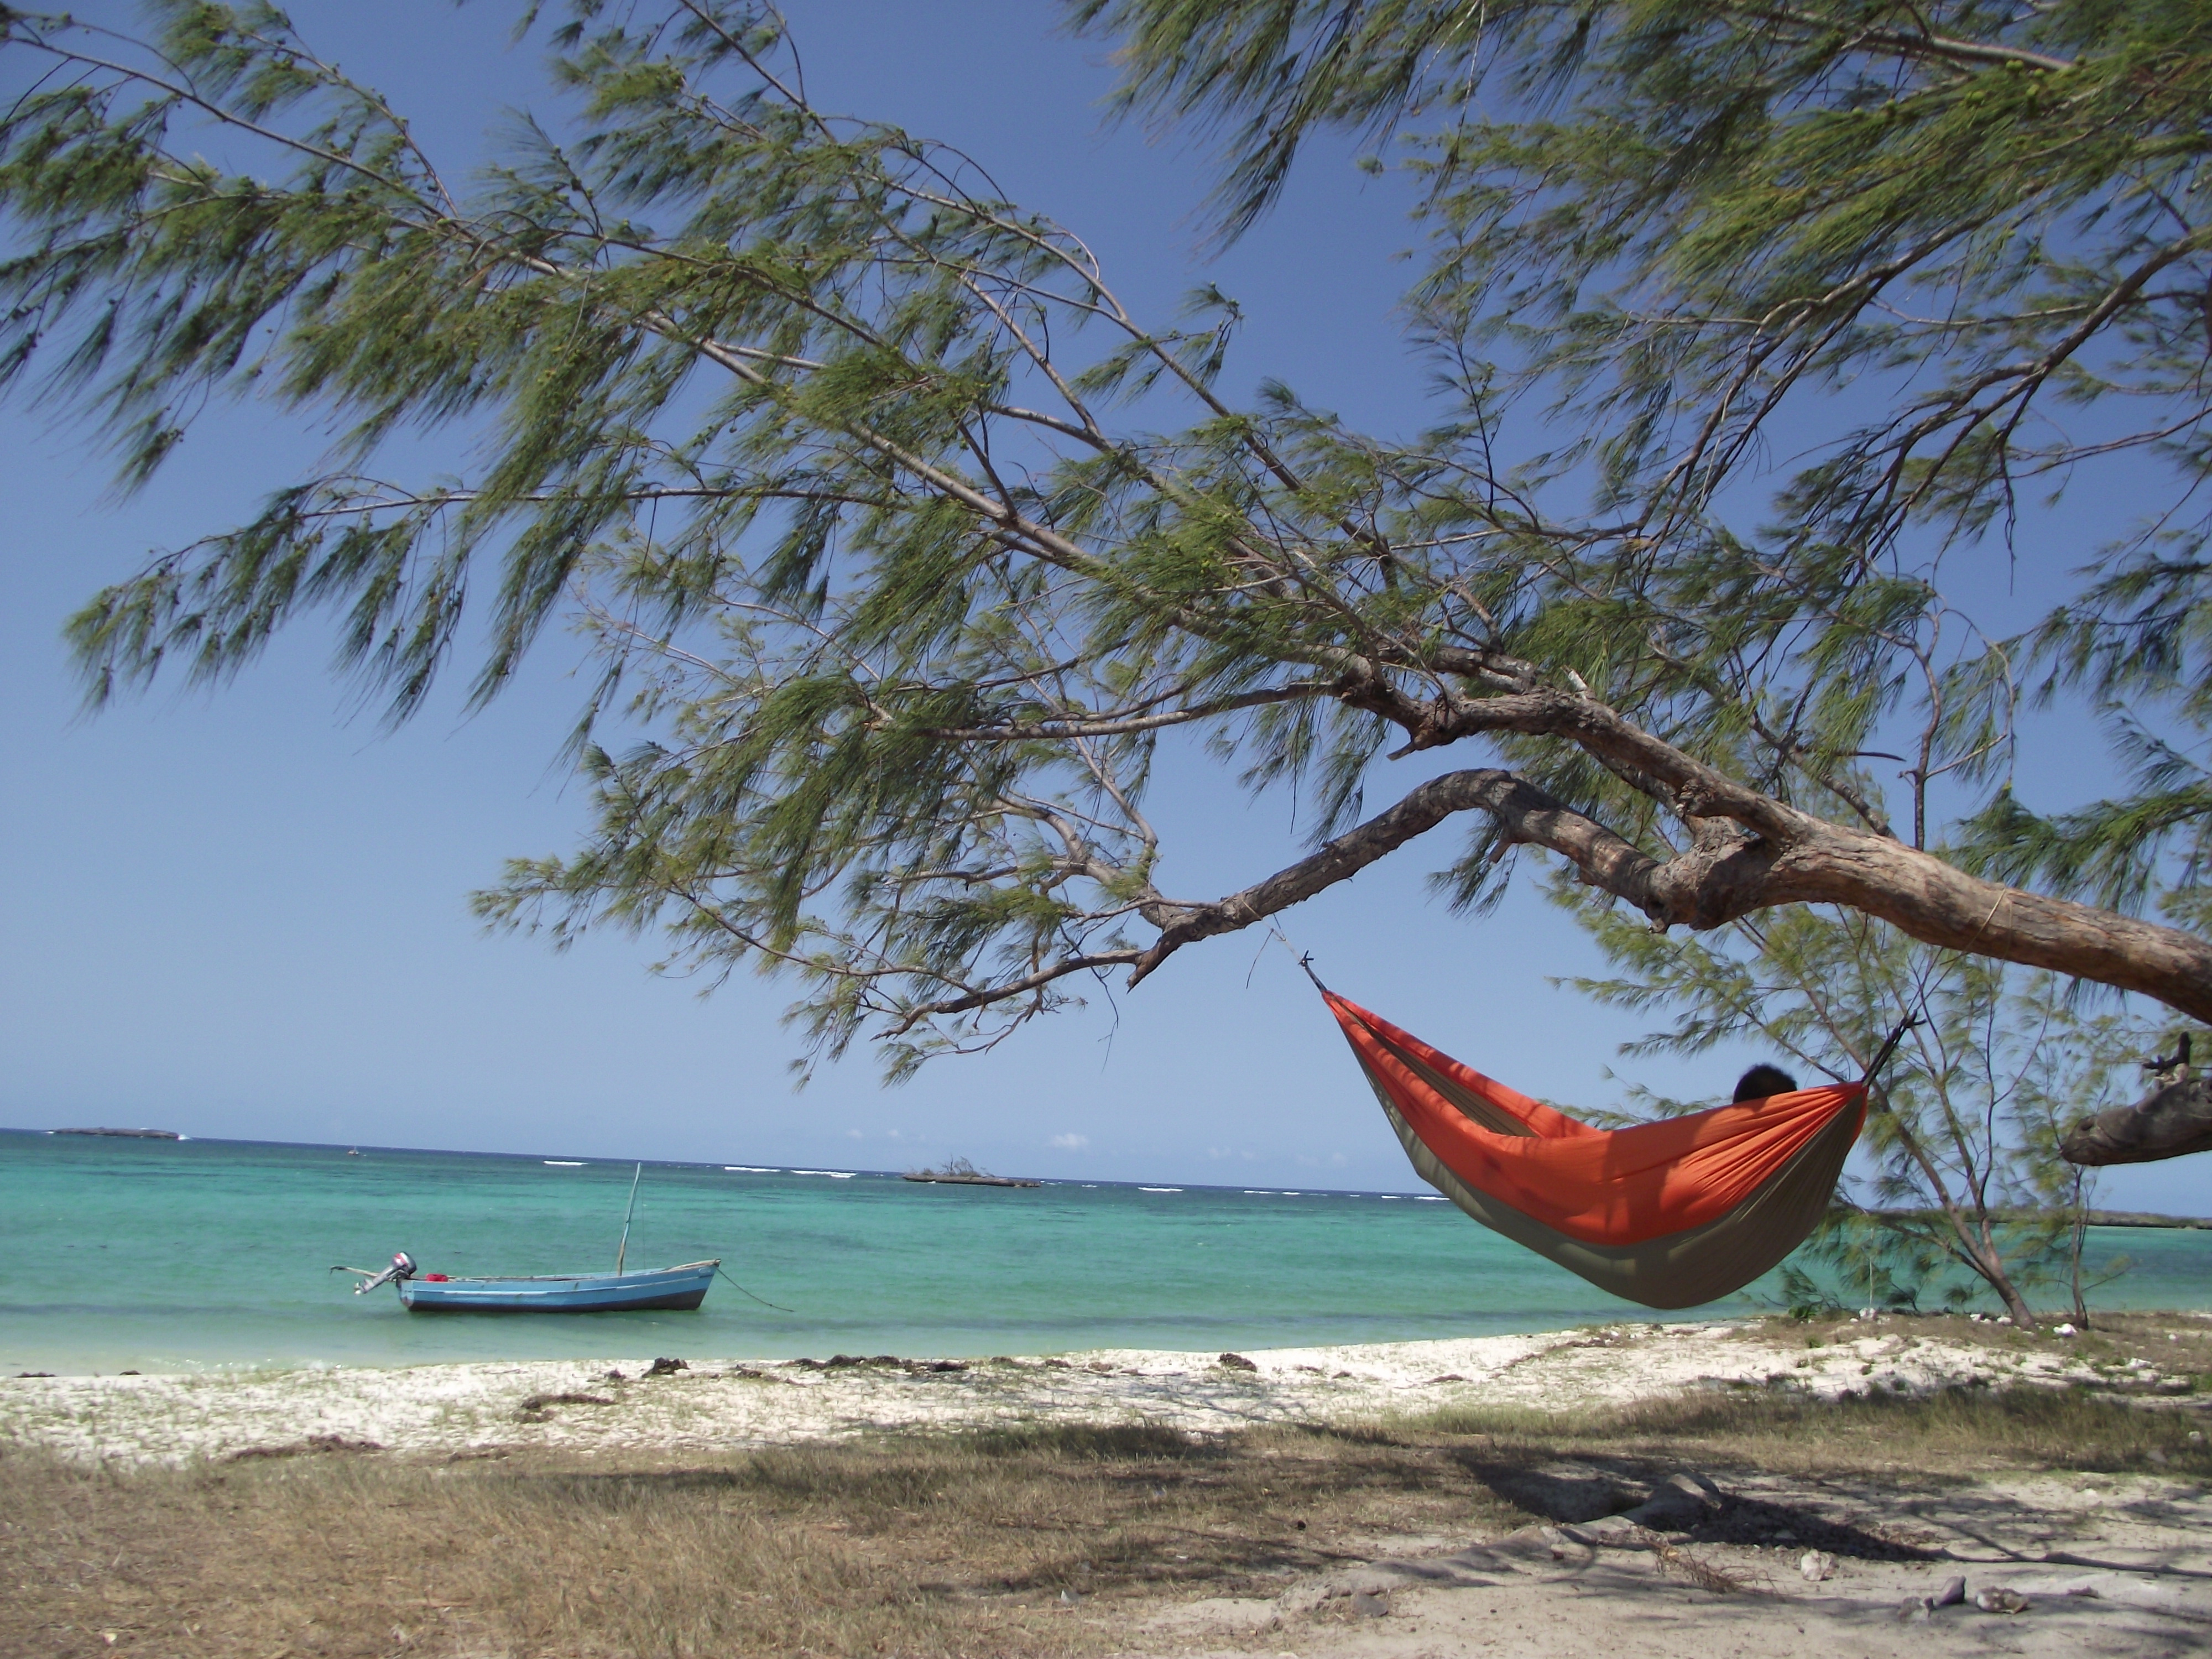
\includegraphics[width=5cm]{articles/Une-boucle-du-cote-vert/DSCF0463.JPG}
\smallbreak

.. et à bientôt dans un autre coin du monde, des suggestions ?

\end{multicols}

\bigskip
\textbf{\textsc{Commentaires}}

 \medskip
Tatid a écrit le 08 déc. 2010 :
\begin{displayquote}
Ouhhhhh, je sens que le retour sur Paris va être dur pour certains :-D
"Après moultes déboires de transports dus à une trop grande méfiance de ma part" => Nan, sérieux, tu deviens méfiant ? C'est pas le dud qu'on connait :-P
Sinon, je n'ai toujours pas reçu ta carte postale, c'est normal ? ;-)
\end{displayquote}

 \medskip
Sonia a écrit le 08 déc. 2010 :
\begin{displayquote}
Majestueux le grand lémure.
Quel dommage que cela soit déjà la fin du voyage, ces petites nouvelles nous faisaient bien rêver.
Vivement les vidéos
Attention ici il neige
\end{displayquote}

 \medskip
Etienne a écrit le 09 déc. 2010 :
\begin{displayquote}
Il neige apparemment tellement que mon vol retour est annulé, me voici bloqué à tana au moins une journée de plus, mais rien ne garanti que l'avion décolle demain.. wait and see..
Brrr, mon avion annulé pour cause de "tempête de neige sur Orly" alors que je suis au soleil, ça laisse vraiment imaginer le choc thermique que je vais prendre. Si j'aurai su j'aurai resté une journée de plus à la plage moi, na !
\end{displayquote}

 \medskip
Rémi a écrit le 09 déc. 2010 :
\begin{displayquote}
Salut Etienne,
Trop bien tes vacances! 
Tu gères!!!! Tu as mis ton hamac, la classe!
Profites bien de la mer turquoise... il neige à Panam!!!!
Fais nous signe dès ton retour pour qu'on aille boire un canon.
\end{displayquote}

 \medskip
Patrick a écrit le 10 juil. 2011 :
\begin{displayquote}
Bravo à vous, 
Partager votre expérience avec les écoliers,collégiens,étudiants,jeunes des cités,afin de croire en eux..
Cordialement à vous.
\end{displayquote}


